 \documentclass{include/protokollclass}
\usepackage{lscape}
\usepackage{graphicx}
\usepackage{colortbl}
\usepackage{amsmath}
\usepackage{float}
% Main File - Based on protokollclass.cls
% Comments are mostly in English (and some in German, concerning the Praktikum)
% ------------------------------------------------------------------------------
% Further files in folder:
%  - include/cmds.tex (for macros and additional commands)
%  - include/kitlogo.pdf (for titlepage)
%  - lit.bib (bibtex bibliography database)
%  - include/titlepage.tex (for layout of titelpage)
% ------------------------------------------------------------------------------
% Useful Supplied Packages:
% amsmath, amssymb, mathtools, bbm, upgreek, nicefrac,
% siunitx, varioref, booktabs, graphicx, tikz, multicol
%
%% ---------------------------------------------
%% |    Informationen über dieses Protokoll    |
%% ---------------------------------------------
\newcommand{\praktikum}{P2}                % P1 oder P2
\newcommand{\semester}{SS18}            % z.B. "WS14/15" oder "SS15"

\newcommand{\wochentag}{Mi}                % Mo, Di, Mi oder Do
\newcommand{\gruppennr}{42}                % Zweistellige Gruppennummer

\newcommand{\nachnamea}{Bernhardt}             % Nachname des ersten Praktikanten
\newcommand{\vornamea}{Felix}               % Vorname des ersten Praktikanten
\newcommand{\nachnameb}{Vosteen}              % Nachname des zweiten Praktikanten
\newcommand{\vornameb}{Lars}              % Vorname des zweiten Praktikanten

\newcommand{\emailadressen}{Felix.Bernhardt@physik.uni-giessen.de, Lars.B.Vosteen@physik.uni-giessen.de}
% optionale Angabe von Emailadresse(n) für den Kontakt mit dem Betreuer

\newcommand{\versuch}{Plasmakristalle} % Name des Versuchs
\newcommand{\versuchsnr}{21}               % bitte die korrekte Nummer dem 
                                           % Arbeitsplatz am Versuchstag 
                                           % entnehmen
\newcommand{\fehlerrechnung}{Ja}         % Ob Fehlerrechnung im Versuch 
                                           % durchgeführt wurde oder nicht

\newcommand{\betreuer}{Dr. Michael Kretschmer}      % Name des zuständigen Betreuers
\newcommand{\durchgefuehrt}{06.07.'18}      % Datum, an dem der Versuch 
                                           % durchgeführt wurde





%% --------------------------------------
%% |    Settings for Word Separation    |
%% --------------------------------------
% Help for separation:
% In German package the following hints are additionally available:
% "- = Additional separation
% "| = Suppress ligation and possible separation (e.g. Schaf"|fell)
% "~ = Hyphenation without separation (e.g. bergauf und "~ab)
% "= = Hyphenation with separation before and after
% "" = Separation without a hyphenation (e.g. und/""oder)

% Describe separation hints here:
\hyphenation
{
    über-nom-me-nen an-ge-ge-be-nen
    %Pro-to-koll-in-stan-zen
    %Ma-na-ge-ment  Netz-werk-ele-men-ten
    %Netz-werk Netz-werk-re-ser-vie-rung
    %Netz-werk-adap-ter Fein-ju-stier-ung
    %Da-ten-strom-spe-zi-fi-ka-tion Pa-ket-rumpf
    %Kon-troll-in-stanz
}





% um die Titelseite per PDF-reader auszufüllen. Vorgefertigte Daten
% können in Datei 'data.tex' modifiziert werden.
%\setboolean{forminput}{true}
% um die Anmerkungen zu den Textfeldern anzeigen zu lassen
%\setboolean{showannotations}{true}
% Erneuern der Seitenzahl in jedem Kapitel
%\setboolean{chapResetPageNumb}{true}
% Einbinden der Kapitelnummer in der Seitenzahl
%\setboolean{chapWiseNumb}{true}
% english or ngerman (new german für neue deutsche Rechtschreibung statt german)
\SelectLanguage{ngerman}





%% -----------------------
%% |    Main Document    |
%% -----------------------
\begin{document}
    % Titlepage und ToC
    \FrontMatter

    % coordinates for background border
\newcommand{\diameter}{20}
\newcommand{\xone}{-15}
\newcommand{\xtwo}{160}
\newcommand{\yone}{15}
\newcommand{\ytwo}{-253}

\newcommand{\hoehea}{60}
\newcommand{\hoeheb}{60}




\begin{titlepage}
    % background border
    \begin{tikzpicture}[overlay]
    \draw[color=gray]  
            (\xone mm, \yone mm)
      -- (\xtwo mm, \yone mm)
    arc (90:0:\diameter pt) 
      -- (\xtwo mm + \diameter pt , \ytwo mm) 
        -- (\xone mm + \diameter pt , \ytwo mm)
    arc (270:180:\diameter pt)
        -- (\xone mm, \yone mm);
    \end{tikzpicture}
    
    % KIT logo
    \begin{textblock}{10}[0,0](4.5,2.5)
        
\includegraphics[width=.15\textwidth]{include/Logo_Fachschaft.png}
    \end{textblock}
    \changefont{phv}{m}{n}    % helvetica
    \begin{textblock}{10}[0,0](5.5,2.2)
        \begin{flushright}
            \Large physikalisches Institut\\Fortgeschrittenenpraktikum
        \end{flushright}
    \end{textblock}
    
    \begin{textblock}{10}[0,0](4.2,3.1)
        \begin{tikzpicture}[overlay]
        \draw[color=gray]
            (\xone mm + 5 mm, -12 mm)
         -- (\xtwo mm + \diameter pt - 5 mm, -12 mm);
        \end{tikzpicture}
    \end{textblock}
    
    \Large
    % Zeile 1
    \begin{textblock}{12}[0,0](3.58,4.4)
        \mytextfield{Prak.}{\praktikum}{0.9cm}{17pt}
                    {P1/P2}{2}{Praktikum}
    \end{textblock}
    \begin{textblock}{12}[0,0](5.53,4.4)
        \mytextfield{Semester}{\semester}{2.6cm}{17pt}
        {z.B. \glqq WS14/15\grqq\ oder \glqq SS15\grqq}{0}{Semester}
    \end{textblock}
    \begin{textblock}{12}[0,0](9.53,4.4)
        \mytextfield{Wochentag}{\wochentag}{1.3cm}{17pt}
                    {Mo/Di/Mi/Do}{2}{Wochentag}
    \end{textblock}
    \begin{textblock}{12}[0,0](12.88,4.4)
       \mytextfield{Gruppennr.}{\gruppennr}{1.06cm}{17pt}
                   {\#\#}{2}{Gruppennummer}
    \end{textblock}
    
    % Zeile 2
    \begin{textblock}{12}[0,0](3.58,4.95)
        \mytextfield{Name}{\nachnamea}{6cm}{17pt}
                    {}{0}{Name1}
    \end{textblock}
    \begin{textblock}{12}[0,0](9.53,4.95)
        \mytextfield{Vorname}{\vornamea}{6cm}{17pt}
                    {}{0}{Vorname1}
    \end{textblock}
    
    % Zeile 3
    \begin{textblock}{12}[0,0](3.58,5.5)
        \mytextfield{Name}{\nachnameb}{6cm}{17pt}
                    {}{0}{Name2}
    \end{textblock}
    \begin{textblock}{12}[0,0](9.53,5.5)
        \mytextfield{Vorname}{\vornameb}{6cm}{17pt}
                    {}{0}{Vorname2}
    \end{textblock}
    
    % Zeile 4
    \begin{textblock}{12}[0,0](3.64,6.05)
       \normalsize\mytextfield{Emailadresse(n)}{\emailadressen}{13.1cm}{10pt}
                              {Optional}{0}{Emailadressen}
    \end{textblock}
    
    % Zeile 5
    \begin{textblock}{12}[0,0](3.58,7)
        \mytextfield{Versuch}{\versuch\ (\praktikum-\versuchsnr)}{9.45cm}{14pt}
                    {z.B. \glqq Galvanometer (P1-13)\grqq\ oder \glqq %
                     Mikrowellenoptik (P2-15)\grqq}{0}{Versuch}
    \end{textblock}
    \begin{textblock}{12}[0,0](12.58,7)
       \mytextfield{Fehlerrech.}{\fehlerrechnung}{1.46cm}{17pt}
                   {Ja/Nein}{4}{Fehlerrechnung}
    \end{textblock}
    
    % Zeile 6
    \begin{textblock}{12}[0,0](3.58,7.55)
        \mytextfield{Betreuer}{\betreuer}{7cm}{17pt}{}{0}{Betreuer}
    \end{textblock}
    \begin{textblock}{12}[0,0](10.82,7.55)
        \mytextfield{Durchgeführt am}{\durchgefuehrt}{2.53cm}{17pt}
                    {TT.MM.JJ}{8}{Durchfuehrung}
    \end{textblock}
    
    % Querstrich
    \begin{textblock}{20}[0,0](0,7.9)\tiny\centering
        Wird vom Betreuer ausgefüllt.
    \end{textblock}
    \begin{tikzpicture}[overlay]
    \draw[color=gray]
        (\xone mm + 5 mm, -95 mm)
     -- (\xtwo mm + \diameter pt - 5 mm, -95 mm);
    \end{tikzpicture}
    
    % Zeile 1
    \begin{textblock}{12}[0,0](3.65,8.57)
        \myTtextfield{Abgabe am}{}{2.5cm}{17pt}
                     {}
    \end{textblock}
    
    % Block 1
    \begin{tikzpicture}[overlay]
    \draw[color=gray]  
        (\xone mm + 10 mm, -107.5 mm)
     -- (\xtwo mm + \diameter pt - 10 mm, -107.5 mm)
     -- (\xtwo mm + \diameter pt - 10 mm, -107.5 mm - \hoehea mm)
     -- (\xone mm + 10 mm, -107.5 mm - \hoehea mm)
     -- (\xone mm + 10 mm, -107.5 mm);
    \end{tikzpicture}
    \begin{textblock}{20}[0,0](3.8,9.2)
        \myTtextfield{Rückgabe am}{}{2.5cm}{17pt}
                     {}
    \end{textblock}
    \begin{textblock}{20}[0,0](8.7,9.2)
        \myTtextfield{Note}{}{2.5cm}{17pt}
                     {}
    \end{textblock}
    
    \begin{textblock}{20}[0,0](4.05,9.6)
        \smash{Begründung:}
    \end{textblock}
    
    
        % lowest text blocks concerning the KIT
    \begin{textblock}{10}[0,0](4,16.8)
        \tiny{Vorlage der Fachschaft Physik der Justus-Liebig-Universität}
    \end{textblock}
    \begin{textblock}{10}[0,0](14,16.75)
        \large{\textbf{www.uni-giessen.de}}
    \end{textblock}
\end{titlepage}
 %\cleardoublepage

    \begingroup \let\clearpage\relax    % in order to avoid listoffigures and
    \tableofcontents                    % listoftables on new pages
    \listoffigures
    \listoftables
    \endgroup
    %\cleardoublepage



    % Contents
    \MainMatter
    
%    \emptychapter[1]{Messprotokoll 1}{} % usage: \emptychapter[page displayed 
                                        %        in toc]{name of the chapter}
%    \pseudochapter[3]{Messprotokoll 2}  % usage: \pseudochapter[number of pages 
                                        %        added]{name of the chapter}
    \setcounter{chapter}{-1}
    \chapter{Zielsetzung}
    \section{Zielsetzung}
In diesem Versuch gilt es, einen Plaskaristall zu erzeugen, zu beobachten und verschiedene Eigenschaften zu bestimmen. Dafür wird mit Argon in einer Niederdruckkammer ein Plasma gezündet. In dieses werden eine Vielzahl Plastikpartikel gegeben, die sich negativ und laden bei geeigneten Umstäden zu einem Kristall anordnen. Mit Hilfe eines Lasers kann dieser ebenenweise mit einer Digitalkamera beobachtet werden.
    \chapter{Theorie}
    \section{Plasma}
Plasma wird oft als der vierte Aggregatzustand bezeichnet. Die Atome liegen hierbei als Ionen vor, die Elektronen und Ionen können sich frei bewegen. Je nach Eigenschaften der Plasmateilchen wird dieses in verschiedene Kategorien eingeteilt:
\begin{itemize}
    \item \textbf{relativistisches Plasma} liegt vor, wenn die kinetische Energie der Elektronen $\approx30\%$ der Lichtgeschwindigkeit beträgt.
    \item Ein \textbf{quantenmechanisches Plasma} liegt vor, wenn die De-Broglie-Wellenlänge der Plasmateilchen größer als der Abstand zwischen den Teilchen ist.
    \item Bei einem \textbf{idealen Plasma} ist die Coulomb-Wechselwirkungsenergie zwischen den Teilchen schwächer als die thermische Energie der Teilchen.
    \item Ist der Ionisationsgrad $\frac{n_i}{n_i+n_g}<<1$, so spricht man von einem \textbf{Niedertemperaturplasma}. Hierbei sind $n_i$ die Dichte der ionisierten- und $n_g$ die Dichte der Neutralgasatome.
\end{itemize}
Für diesen Versuch wird ein nicht-relativistisches, klassisches, stark gekoppeltes 
Niedertemperaturplasma benötigt.

\section{Plasmakristall}
Die Plasmateilchen sind frei beweglich, sie können daher keine Kristallstrutktur bilden. Um diese zu erzeugen wird ein sogennantes \textbf{komplexes Plasma} benötigt: Zum Plasma werden kleine, feste Kügelchen (Radius $\approx1\mu m$) zugesetzt. Die Partikel laden sich daraufhin durch Stöße mit den freien Elektronen des Plasmas auf. Durch die Coulomb\,-\,Wechselwirkung zwischen diesen stark geladenen Kügelchen können diese unter richtigen Randbedingungen in einen geordneten Zustand gebracht werden und der Plasmakristall ensteht. Durch ein elektrisches Feld kann der Kristall in Schwebe gehalten, und mit einem Laser beobachtet werden,
\\
Zusätzlich wirken aufgrund des Neutralgases Reibungskräfte auf den Kristall. Zudem kann Thermospherese auftreten: Dabei werden die Teilchen entlang des Temperaturgradieten im Plasma bewegt.

\section{Struktur des Kristalls}
Ein Kristall zeichnet sich durch Fernordnung aus, d.h. die Abstände der Atome (in unserem Fall der Plastikkügelchen) sind periodisch. Die Paarkorrelationsfunktion $g(\textbf{r})$ ist ein Maß für die Wahrscheinlichkeit einer Fernordnung: 
$$
    g(\textbf{r})=\Big\langle\frac{1}{N}\sum_{i\neq j}^{N}\delta(\textbf{r}-(\textbf{r}_i-\textbf{r}_j)\Big\rangle
$$
Die Funktion gibt also den Erwartungswert an, dass sich im Abstand r von einem Teilchen i ein anderes Teilchen j befindet. Liegt Fernordnung vor und zeichnet man die Funktion g gegen r auf, so sind daher periodische Peaks zu finden. Die Struktur muss nicht im gesamten Kristall dieselbe sein: Es können sich auch Domänen bilden, d.h. das verschiedene \glqq Abschnitte\grqq{} des Kristalls unterschiedliche Strukturen besitzen können.
\\
Im Verlauf der Auswertung wird die Struktur mithilfe der Local-Order-Analyse durchgeführt. Hierfür werden Bond-Order-Parameter (numerisch) berechnet:
$$
    q_l(\textbf{r}_i)=\sqrt{\frac{4\pi}{2l+1}\sum_{m=-l}^{l}|q_{lm}(\textbf{r}_i)|^2}
$$
Mit
$$
    q_{lm}(\textbf{r}_i)=\frac{1}{N}\sum_{j=1}^{N}Y_{lm}(\Theta(\textbf{r}_i-\textbf{r}_j),\Phi(\textbf{r}_i-\textbf{r}_j))
$$
Mithilfe dieser Funktionen könnnen verschiedene Domänenstrukturen bestimmt werden.
    \chapter{Auswertung}
    \section{Abbildungsmaßstab des Kamerasystems}
Bevor das Plasma gezündet wird, muss der Abbildungsmaßstab der Messvorrichtung bestimmt werden. Hierzu vermessen wir den Abstand der unteren Elektrode zum Rand der Kammer bei verschiedenen Kamerapositionen und lassen uns mithilfe des Programmes \glqq uEyeCockpit\grqq{} die Länge dieser Distanz in Pixeln ausgeben. Damit erhalten wir:

\begin{table}[ht]
    \centering
    \begin{tabular}{c|c}
         Kameraabstand/Zoll& Distanz/Pixel \\\hline
         0.8 & 34 \\
         0.0 & 914 \\
    \end{tabular}
    \caption{Bestimmung des Abbildungsmaßstabes}
    \label{tab:abbmaß}
\end{table}

Der Abbildungsmaßstab A ergibt sich dann zu:
$$
    A=\frac{(0.8-0.0)Zoll*2,54*10^4\frac{cm}{Zoll}}{(914-34)Pixel}=23,09\frac{\mu m}{Pixel} 
$$

\section{Herstellung des Kristalls}
Nun leiten wir Argon-Gas in die Kammer; Dabei wird der Druck auf 40\,Pa gesetzt. Ab einer RF-Spannug von 1,15\,V zündet das Plasma. Die Spannung wird nun auf 0,15\,V reduziert, wobei der Plasmazstand des Gases erhalten bleibt. Anschließend werden die Plastikpartikel aus Melamin-Formaldehyd mit einem Dispenser in die Kammer gebracht. Die Partikel ordnen sich nach einer Zeit von 1-2\,min an und bleiben (in guter Näherung) in Position; Der Plasmakristall wurde hergestellt. An sämtlichen Rändern des Kristalls bewegen sich die Partikel recht stark, nur im inneren der Struktur sind die Teilchen fix. Im unteren Bereich des Kristalls haben sich die Plastikkügelchen \glqq geklumpt\grqq{} (große Punkte im Bild); Durch das erhöhte Gewicht werden sie nach unten gezogen (siehe Abbildung \ref{fig:groWo}).


\begin{figure}[ht]
    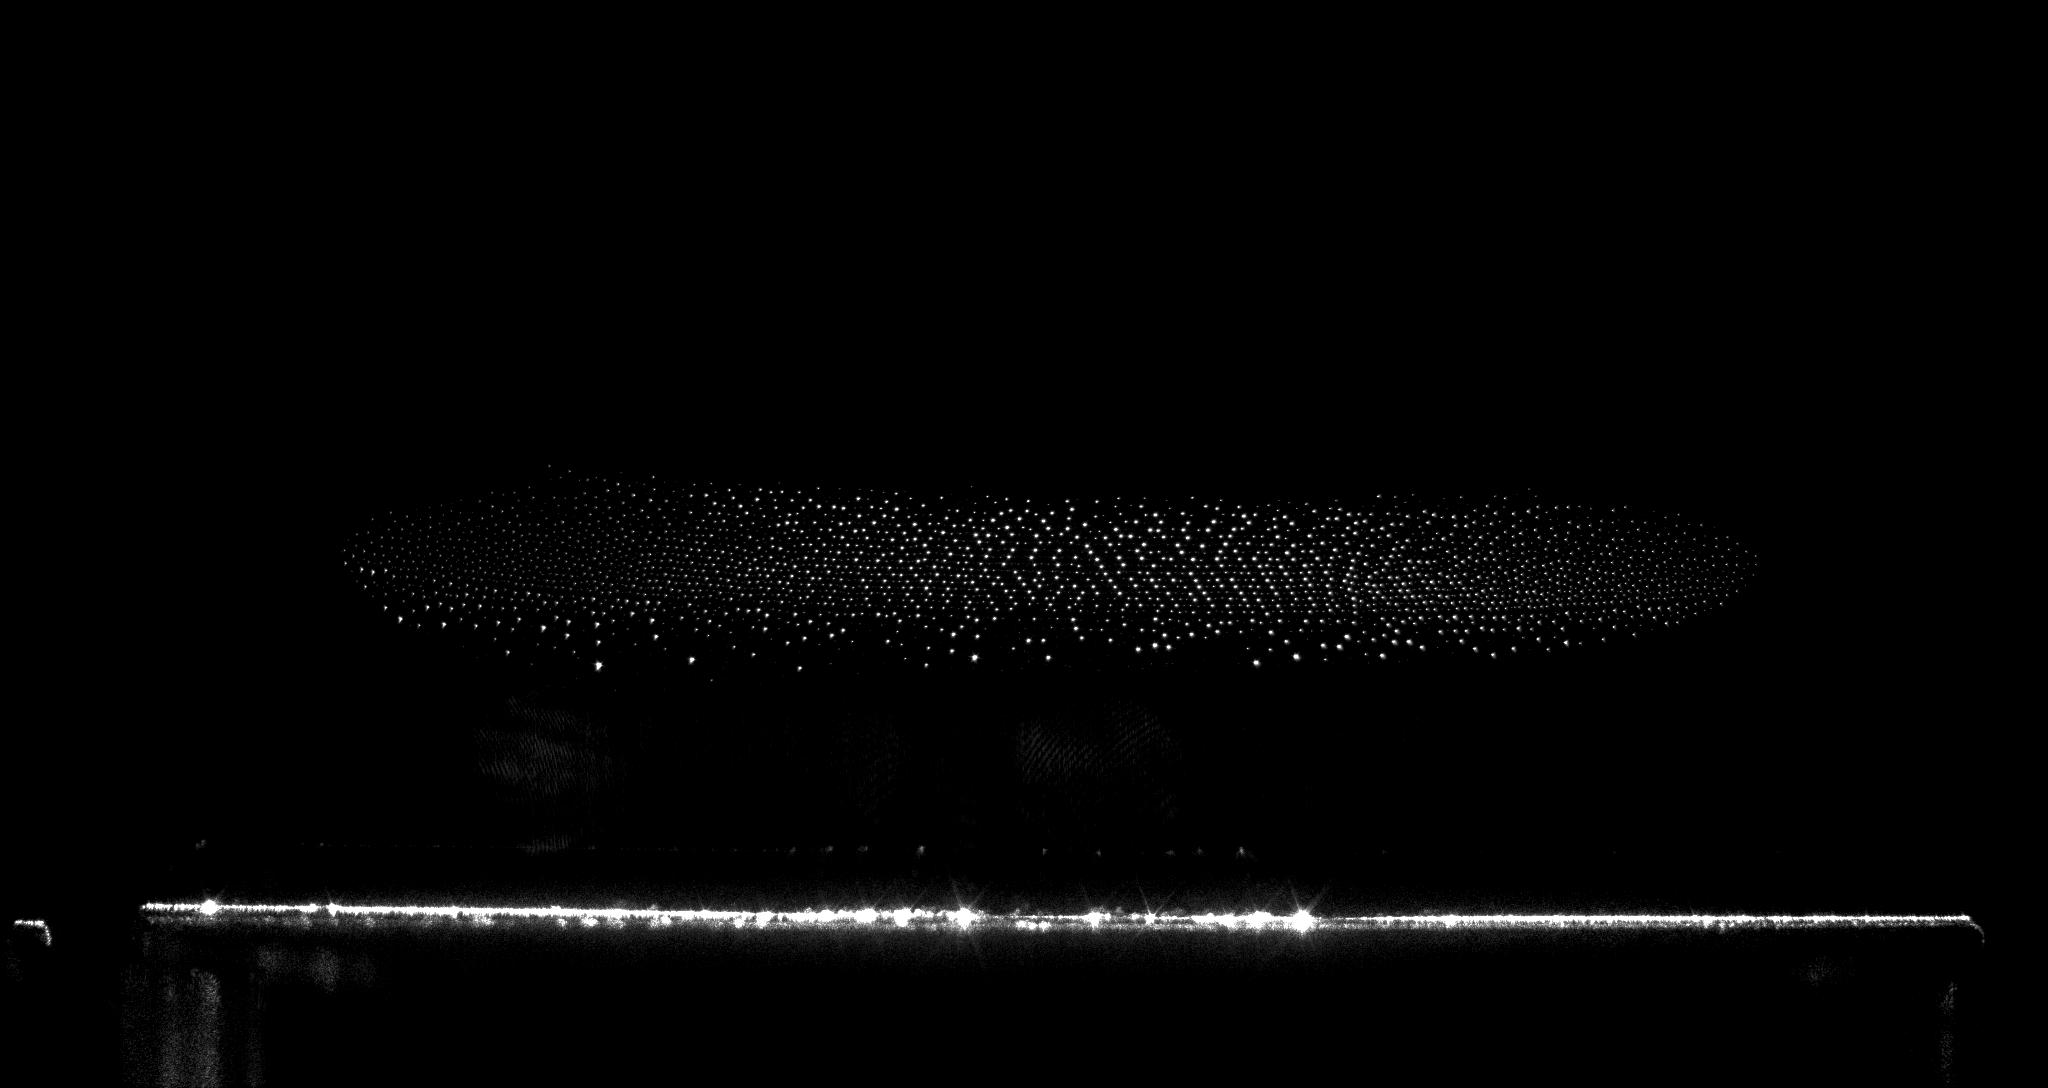
\includegraphics[scale=0.208]{data/Groesse-Teilchenwolke.jpg}
    \caption{Plasmakristall}
    \label{fig:groWo}
\end{figure}

%2. Dimensionen des Kristalls (vorzugsweise in μm) bestimmen:
%a) Gitterabstand in horizontaler (x) und vertikaler (y) Richtung (Messung an mehreren Stellen: Mitte unten, Mitte halbe Höhe, halber Radius unten, halber Radius halbe Höhe. Wenn möglich messen und mitteln Sie über einige (ca. 4-6) Teilchenabstände.),
%b) Breite und Höhe der Teilchenwolke (approximieren Sie den Schnitt durch die Teilchenwolke durch ein sinnvoll gewähltes Rechteck),
%c) Gesamtteilchenzahl (verwenden Sie dazu die von Ihnen gemessenen Teilchenabstände in x und y unter der vereinfachenden Annahme einer kubischen Einheitszelle. Sie können anneh- men, dass z = x und dass Sie den mittleren Schnitt durch die zylindersymmetrische Teilchenwolke sehen). Lassen Sie Ihre Werte vor Ort vom Betreuer prüfen!

\section{Vermessung des Kristalls}
Die Tabellen (\ref{tab:mess-anz} und \ref{tab:anz}) der genauen Messwerte befinden sich im Anhang auf Seite \pageref{tab:mess-anz}. Nachfolgend stehen gerundete Werte; gerechnet wurde mit möglichst genauen.
\subsection{Gitterabstand}
Der ermessene gemittelte horizontale Gitterabstand beträgt $\sim8\,$ Pixel $\approx\,0,19\,$mm. In vertikaler Ausrichtung maßen wir $\sim6\,$Pixel $\approx\,0,15\,$mm.  
\subsection{Ausmaße}
Außmessen ergab eine Breite von $\sim1410\,\text{Pixel}\approx32,4\,mm$ und eine Höhe von $\sim120\,\text{Pixel}\approx2,8\,mm$ des Kristalls. Nebeneinander existieren also $\sim170$ Teilchen: übereinander $\sim20$. 
\subsection{Teilchenanzahl}
Aus obenstehenden Angaben lässt sich unter der Prämisse der rotationssymmetrischen Gleichverteilung und Zylinderartigkeit des Kristalls, die Anzahl der Teilchen in der Wolke bestimmen: $$\bigg(\frac{\text{horizontale Anzahl}}{2}\bigg)^2\cdot\pi\cdot\text{vertikale Anzahl} \approx 425\,000$$



%3. Hausaufgabe: Abschätzung der Partikelladung Q (bei Vernachlässigung der Teilchendichte n d , Angabe bitte in Coulomb und Elementarladungen), des elektrischen Felds E zur Levitation der Partikel, der Debye-Länge λ D , des Coulomb-Kopplungsparameters Γ und des effektiven Parameters Γ eff . (Tipp: Verwenden Sie die Formeln aus der Anleitung. Beachten Sie, dass diese zum Teil in cgs-Einheiten notiert sind!) Sind die Werte plausibel? Kommentieren Sie! Angaben: Teilchenradius a = 1, 0 μm, kT e = 3 eV, kT i = 0, 03 eV, Dichte von Melamin- Formaldehyd 1510 kg/m 3 , F n = F i = F th = 0, T d = 300 K, n i = 10 9 cm −3 .

Mit den folgenden Werten (\cite{1},\cite{TR}) sollen weitere Abschätzungen gemacht werden.

\begin{align}
\text{Partikelradius: }a &= 1\,\mu m \notag\\
\text{Ionentemperatur: }k_BT_i &= 0, 03\,eV\notag\\
\text{Elektronentemperatur: }k_BT_e &= 3\,eV\notag\\
\text{Dichte von Melamin-Formaldehyd: }\rho &= 1510\,\frac{\text{kg}}{\text{m}^3}\notag\\
\text{kinetische Partikeltemperatur: }T_d &= 300\,\text{K}\notag\\
\text{Materialkonstante B: }B&=0,73\notag\\
\text{Dichte der Ionen: }n_i &= 10^9\,\frac{1}{\text{cm}^3}\notag\\
\text{Masse Argon: }M_{Ar}&=39,95\,u\notag\\
\text{F}_n = \text{F}_i = \text{F}_{th} &= 0\notag\\
\text{Erdbeschleunigung: }g&=9,81\,\frac{m}{s^2}\notag\\
\text{Elektronenladung: }e&=1,602\cdot 10^{-19}\,\text{C}\notag\\
\text{Boltzmann-Konstante: }k_B&=1,3807\cdot 10^{-23}\,\frac{J}{K}\notag\\
\text{Dielektrizitätskonstante: }\epsilon_0&=8,85\cdot 10^{-12}\,\frac{As}{Vm}\notag\\
\text{Elektronenmasse: }m_e&=9,11\cdot v10^{-31}\,\text{C}\notag\\
\end{align}


Die Ladung der Partikel Q erhalten wir dann zu:
$$
    Q=Z\cdot e=B\frac{4\pi\epsilon_0ak_BT_e}{e}ln\Big( \sqrt{\frac{T_em_e}{T_iM_{Ar}}}\Big)=-4,97\cdot 10^3\,e=-7,96\cdot 10^{-16}C
$$
  
Um diese Partikel in Schwebe zu halten wird folgende Feldstärke benötigt (Die Plastikkugeln werden als perfekte Kugeln angenähert):
$$
    E=\frac{F}{Q}=\frac{M\cdot g}{Q}=\frac{\rho \frac{4}{3}\pi a^3\cdot g}{Q}=-77,92\,\frac{V}{m}
$$

Die Debye-Wellenlänge ergibt sich zu:
$$
    \lambda_D=\sqrt{\frac{\epsilon_0k_BT_i}{e^2n_i}}=40,7\mu m
$$

Um den Coulomb-Kopplungsparameter $\Gamma$ zu bestimmen benötigen wir zuerst den Partikelabstand\footnote{Diesen mitteln wir aus horizontalem und vertikalen Abständen um eine Richtungsabhängigkeit des Parameters zu vermeiden.} $\Delta$:
$$
    \Delta=\frac{\tilde{x}+\tilde{y}}{2}\approx170\,\mu m
$$

$$
    \Rightarrow\Gamma=\frac{Q^2}{4\pi\epsilon_0\Delta k_BT_d}\approx 8093
$$

Der effektive Coulomb-Kopplungsparameter berücksichtigt zusätzlich die Debye Wellenlänge und den Partikelabstand:
$$
    \Gamma_{eff}=\Gamma\cdot exp\Big(-\frac{\Delta}{\lambda_D}\Big)\approx124
$$ 
Wir haben also mit ein stark gekoppeltes Plasma vorliegen ($\Gamma>1$).

\section{Laserscan}

\begin{figure}[ht]
    
\includegraphics[width=\textwidth]{data/Video0001.jpg}
    \caption{Bildausschnitt des Laserscans}
    \label{fig:videobildausschnitt}
\end{figure}
\begin{figure}[ht]
    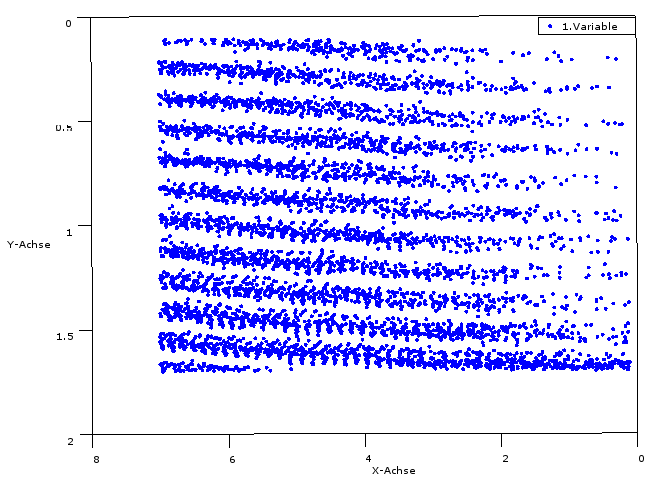
\includegraphics[width=\textwidth]{data/dreiDmodell.PNG}
    \caption{Ergebnis des Laserscans}
    \label{fig:scanerg}
\end{figure}

Nach Wahl eines geigneten Bildausschnitts (siehe Abbilddung \ref{fig:videobildausschnitt}) wird ein Laserscan durchgeführt. Die Ergebnisse des Scans sind in zwei der resultierenden drei Dimensionen in Abb. \ref{fig:scanerg} dargestellt. Die Abstände der Teilchen haben wir ebenfalls bestimmt, das zugehörige Histogramm ist in Abbildung \ref{fig:Abstand} zu finden.

\begin{figure}[ht]
    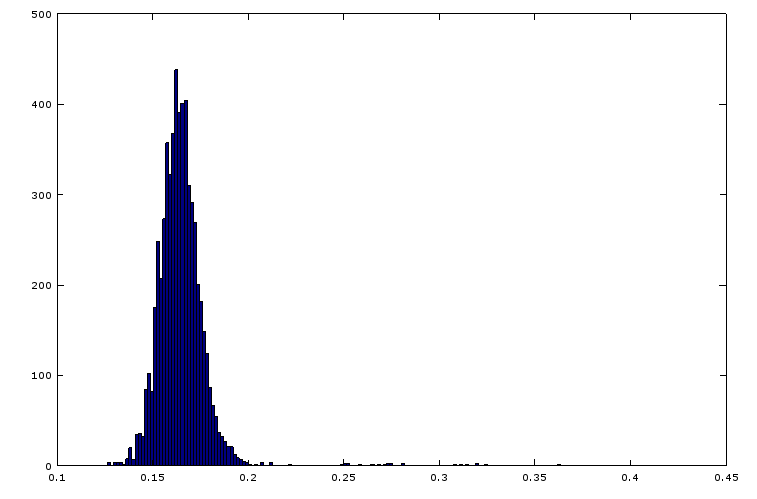
\includegraphics[width=\textwidth]{data/histogramm.PNG}
    \caption{Histogramm der Teilchenabstände}
    \label{fig:Abstand}
\end{figure}

Die Verteilung der Abstände ist recht scharft auf einen Bereich zwischen 0,15-0,18mm begrenzt. Für einen idealen Kristall sollten sich $\delta$-Peaks ergeben. Die Paarkorrelationsfunktion g kann in Abbildung \ref{fig:gr} gesehen werden: Die Fernordnung der Struktur ist dort deutlich zu erkennen.

\begin{figure}[ht]
    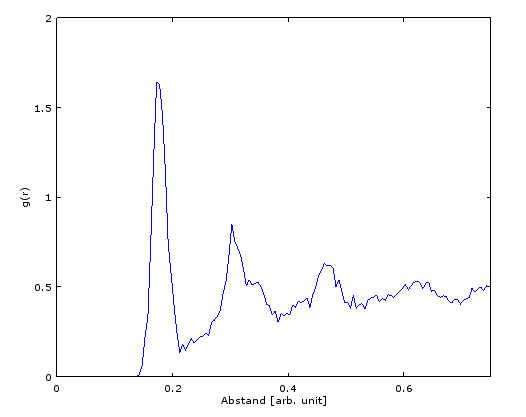
\includegraphics[width=\textwidth]{data/g(r).PNG}
    \caption{Paarkorrelationsfunktion des Kristalls}
    \label{fig:gr}
\end{figure}


\section{Bestimmung des vorliegenden Gittertypes}

Wir betrachten hauptsächlich kubisch\,-\,flächenzentrierte (FCC), kubisch-raumzentrierte (BCC) und hexagonale (HCP) Gitter. Für alle diese Gittertypen wird nun die Paarkorrelationsfunktion g, sowie der Teilchenabstand berechnet. Sämtliche Abbildungen befinden sich auf Seiten \pageref{fig:bccxy}-\pageref{fig:hcpg} im Anhang.
\\
Zur Bestimmung welche Kristallstruktur vorliegt, werden die Bond-Order-Parameter q4 und q6 der idealen Strukturen berechnet und mit den experimentell erhaltenen verglichen. Die berechneten, idealen Parameter sind in Tabelle \ref{tab:bondorder} gegeben.

\begin{table}[ht]
    \centering
    \begin{tabular}{c|ccc}
         & BCC & FCC & HCP \\\hline
         q4 &  0.509 & 0.191 & 0.097\\
         q6 &  0.629 & 0.575 & 0.485\\
    \end{tabular}
    \caption{Bond-Order-Parameter der idealen Strukturen}
    \label{tab:bondorder}
\end{table}

Die Bond-Order Parameter unseres Kristalls werden nun bezüglich ihrer Häufigkeit geplottet: Rot steht für häufig, blau für selten auftretende Werte. Die Abbildungen können in \ref{fig:08} und \ref{fig:12} gefunden werden. Es werden hierfür einmal die 8- und einmal die 12-nächsten Nachbarn betrachtet.

\begin{figure}[ht]
    \centering
    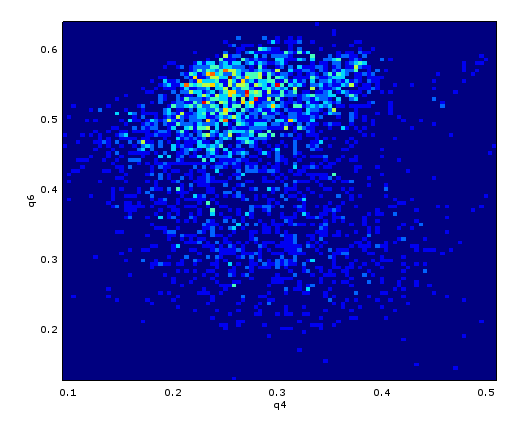
\includegraphics[scale=0.75]{data/rotationinvarianz08.PNG}
    \caption{Bond-Order-Parameter; 8 Nachbarn}
    \label{fig:08}
\end{figure}

\begin{figure}[ht]
    \centering
    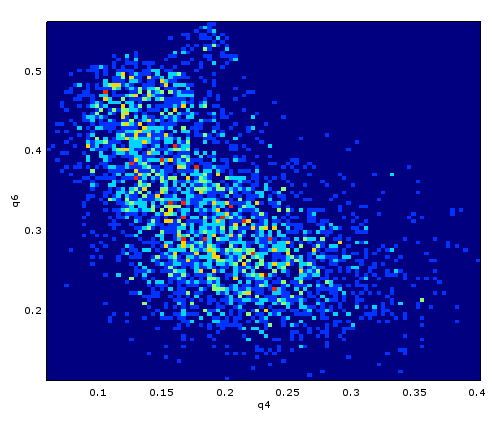
\includegraphics[scale=0.75]{data/rotationinvarianz12.PNG}
    \caption{Bond-Order-Parameter; 12 Nachbarn}
    \label{fig:12}
\end{figure}

In Abbildung \ref{fig:08} lässt sich ein Maximum bei etwa [q4=0,25; q6=0,55] erkennen. Dieser Bereich lässt sich keiner der gegeben Strukturen zuordnen. Dafür wird das Ergebniss beim betrachten der 12-nächsten Nachbarn in Abbildung \ref{fig:12} deutlicher: Es lassen sich eindeutig Bereiche der HCP-Struktur zuordnen, außerdem ist eine kleine Domäne der FCC-Struktur zu finden (vgl. mit Tabelle \ref{tab:bondorder}). BCC-Domänen liegen hingegen nicht vor.

\section{Grenzbereiche}
Abschließend soll die Struktur der Plastikteilchen bei Änderungen der Spannung und des Druckes untersucht werden. Als Ausgagssrtuktur wird ein Druck von 40\,Pa und eine RF-Spannung von 0,15\,eV verwendet (siehe als Vergleich Bild \ref{fig:groWo}).

\subsection{Änderung des Druckes}
Wir verringern nun den Druck von 40\,Pa auf 14\,Pa. Ab 32\,Pa beginnen die Partikel des Kristalls in den unteren Schichten zu oszillieren, ab 24\,Pa ist die Struktur nicht mehr zu erkennen; Der Kristall ist \glqq geschmolzen\grqq{}. Durch Verringerung des Druckes wird die Partikelladung der Teilchen und damit der Parameter $\Gamma$ kleiner. Zudem verringert sich die Reibung der Partikel an den Gasatomen, wodurch die kinetische Energie der Partikel weiter erhöht wird. Dadurch wird die Kristallstruktur aufgebrochen.

\begin{figure}[ht]
    \centering
    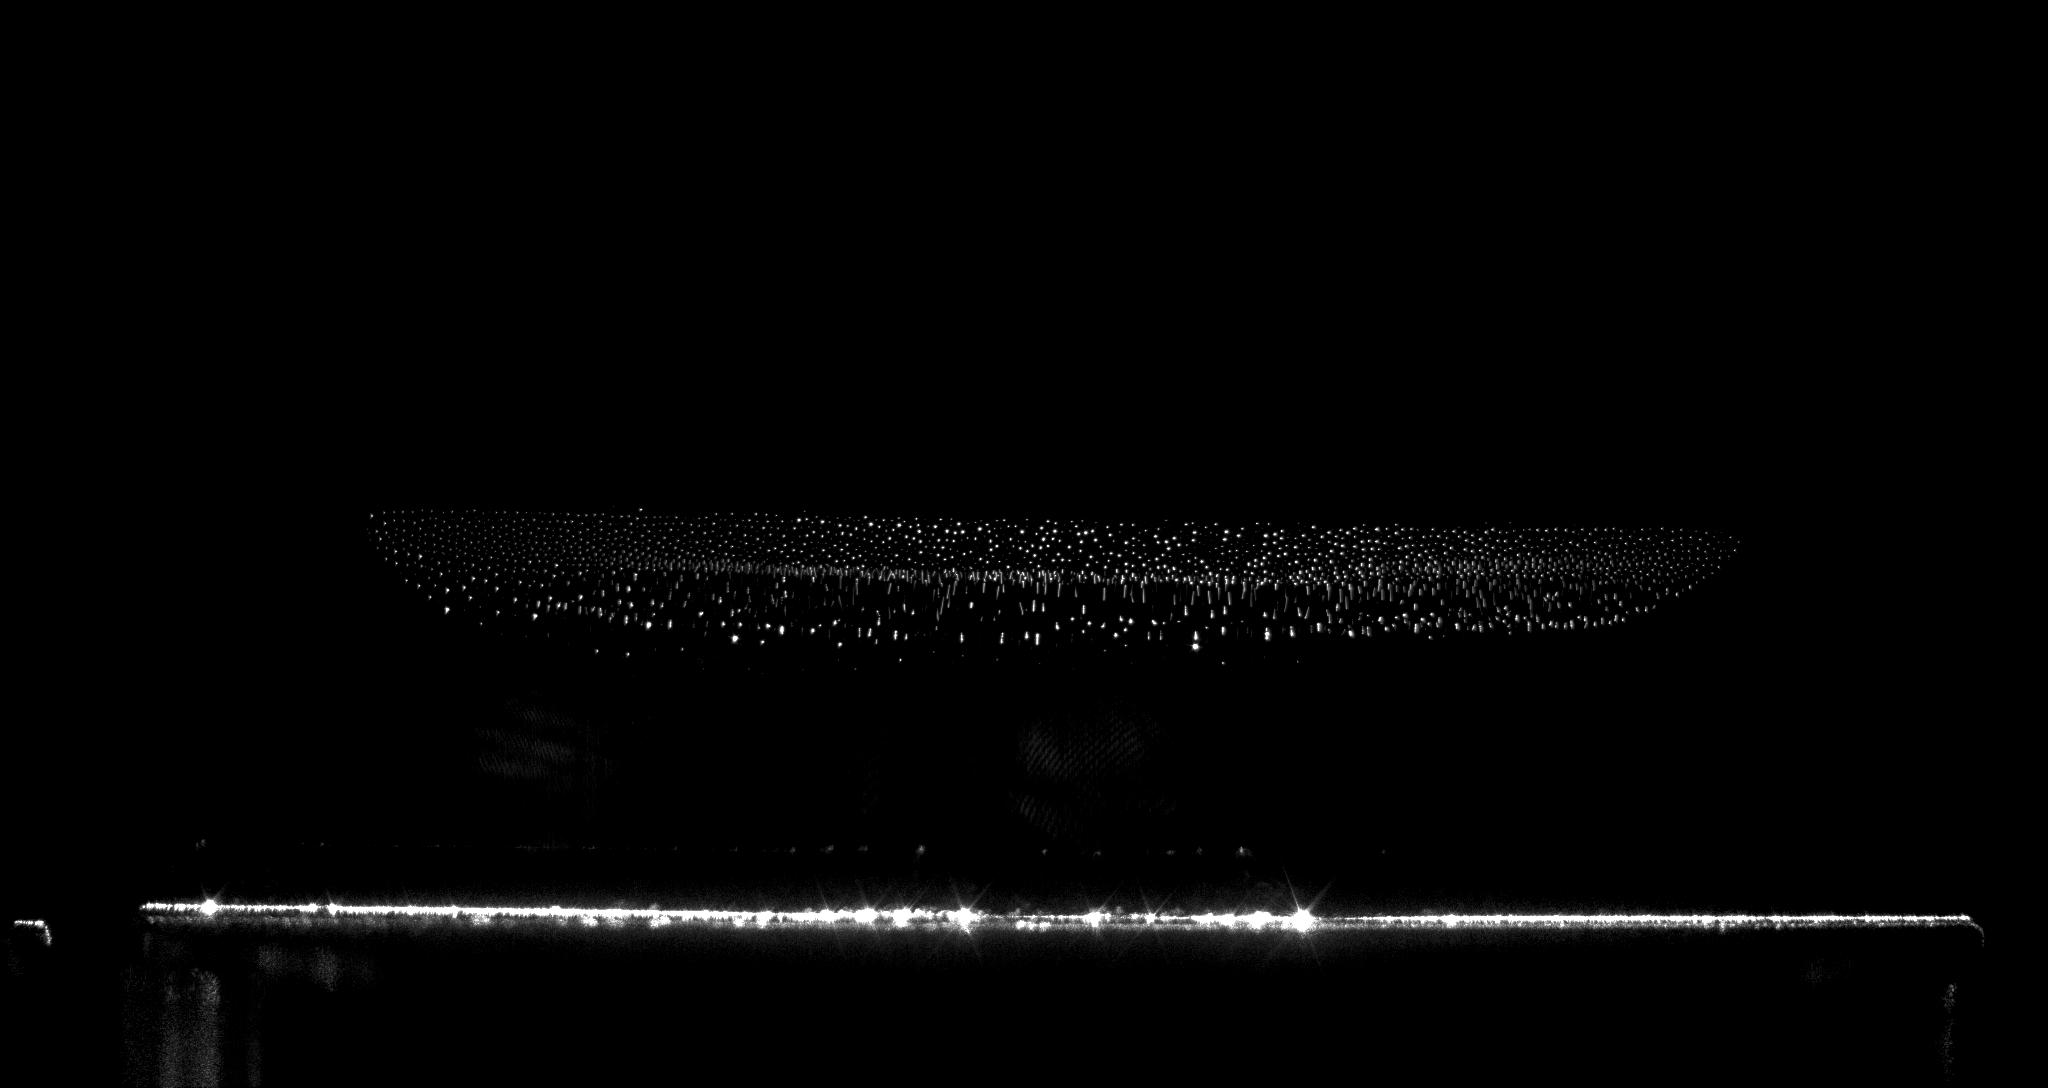
\includegraphics[width=\textwidth]{data/32pa.jpg}
    \caption{Partikelwolke bei 32\,Pa}
    \label{fig:32pa}
\end{figure}

\begin{figure}[ht]
    \centering
    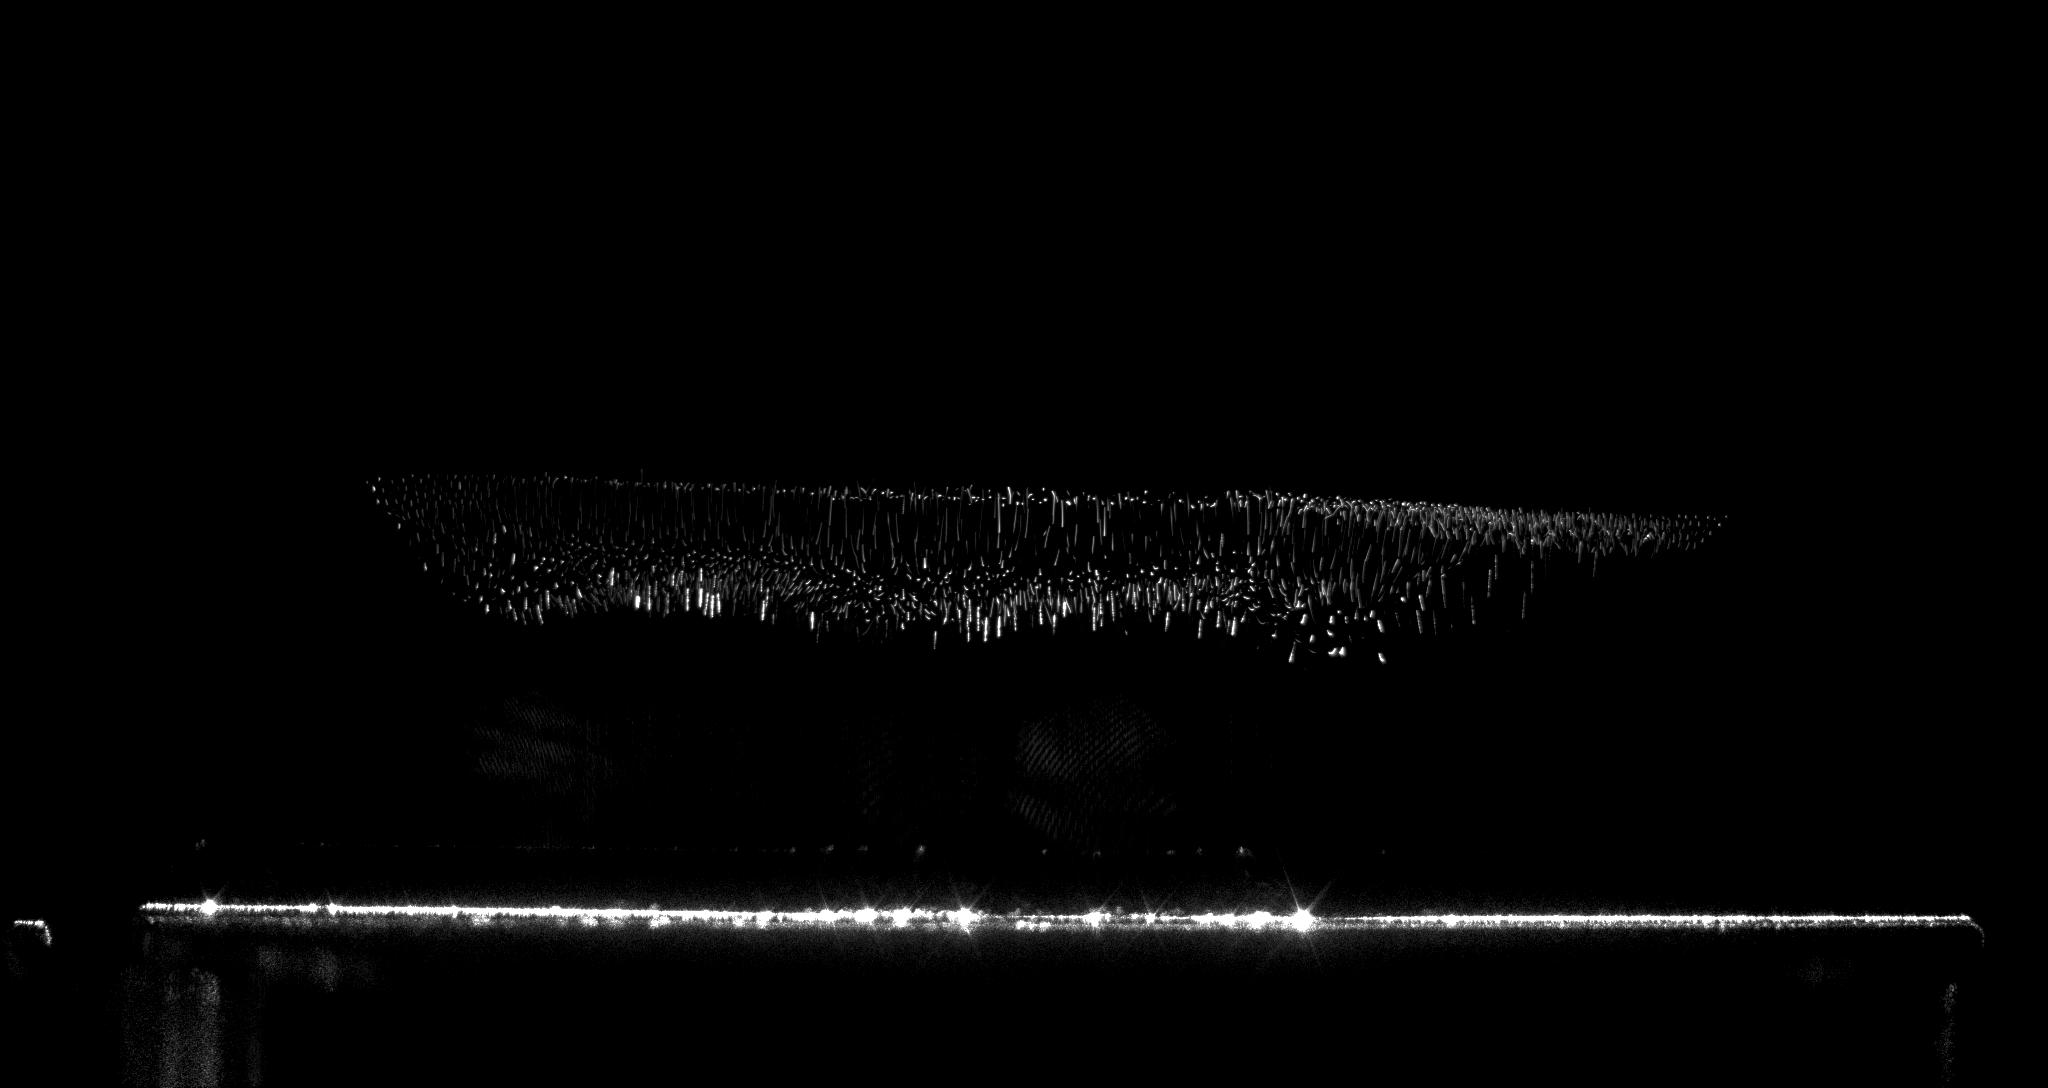
\includegraphics[width=\textwidth]{data/24pa.jpg}
    \caption{Partikelwolke bei 24\,Pa}
    \label{fig:24pa}
\end{figure}

\subsection{Änderung der Spannung}
Bei 40\,Pa erhöhen wir nun die Spannung von 0,15\,V auf 1,5\,V. Der Kristall wird dabei vertikal zusammengedrückt und horizontal gestreckt. Hierbei ändern sich die Teilchenabstände in vertikaler Richtung von etwa 6,25 zu 6 Pixeln, in horizontaler Richtung bleibt der Teilchenabstand konstant.

\begin{figure}[ht]
    \centering
    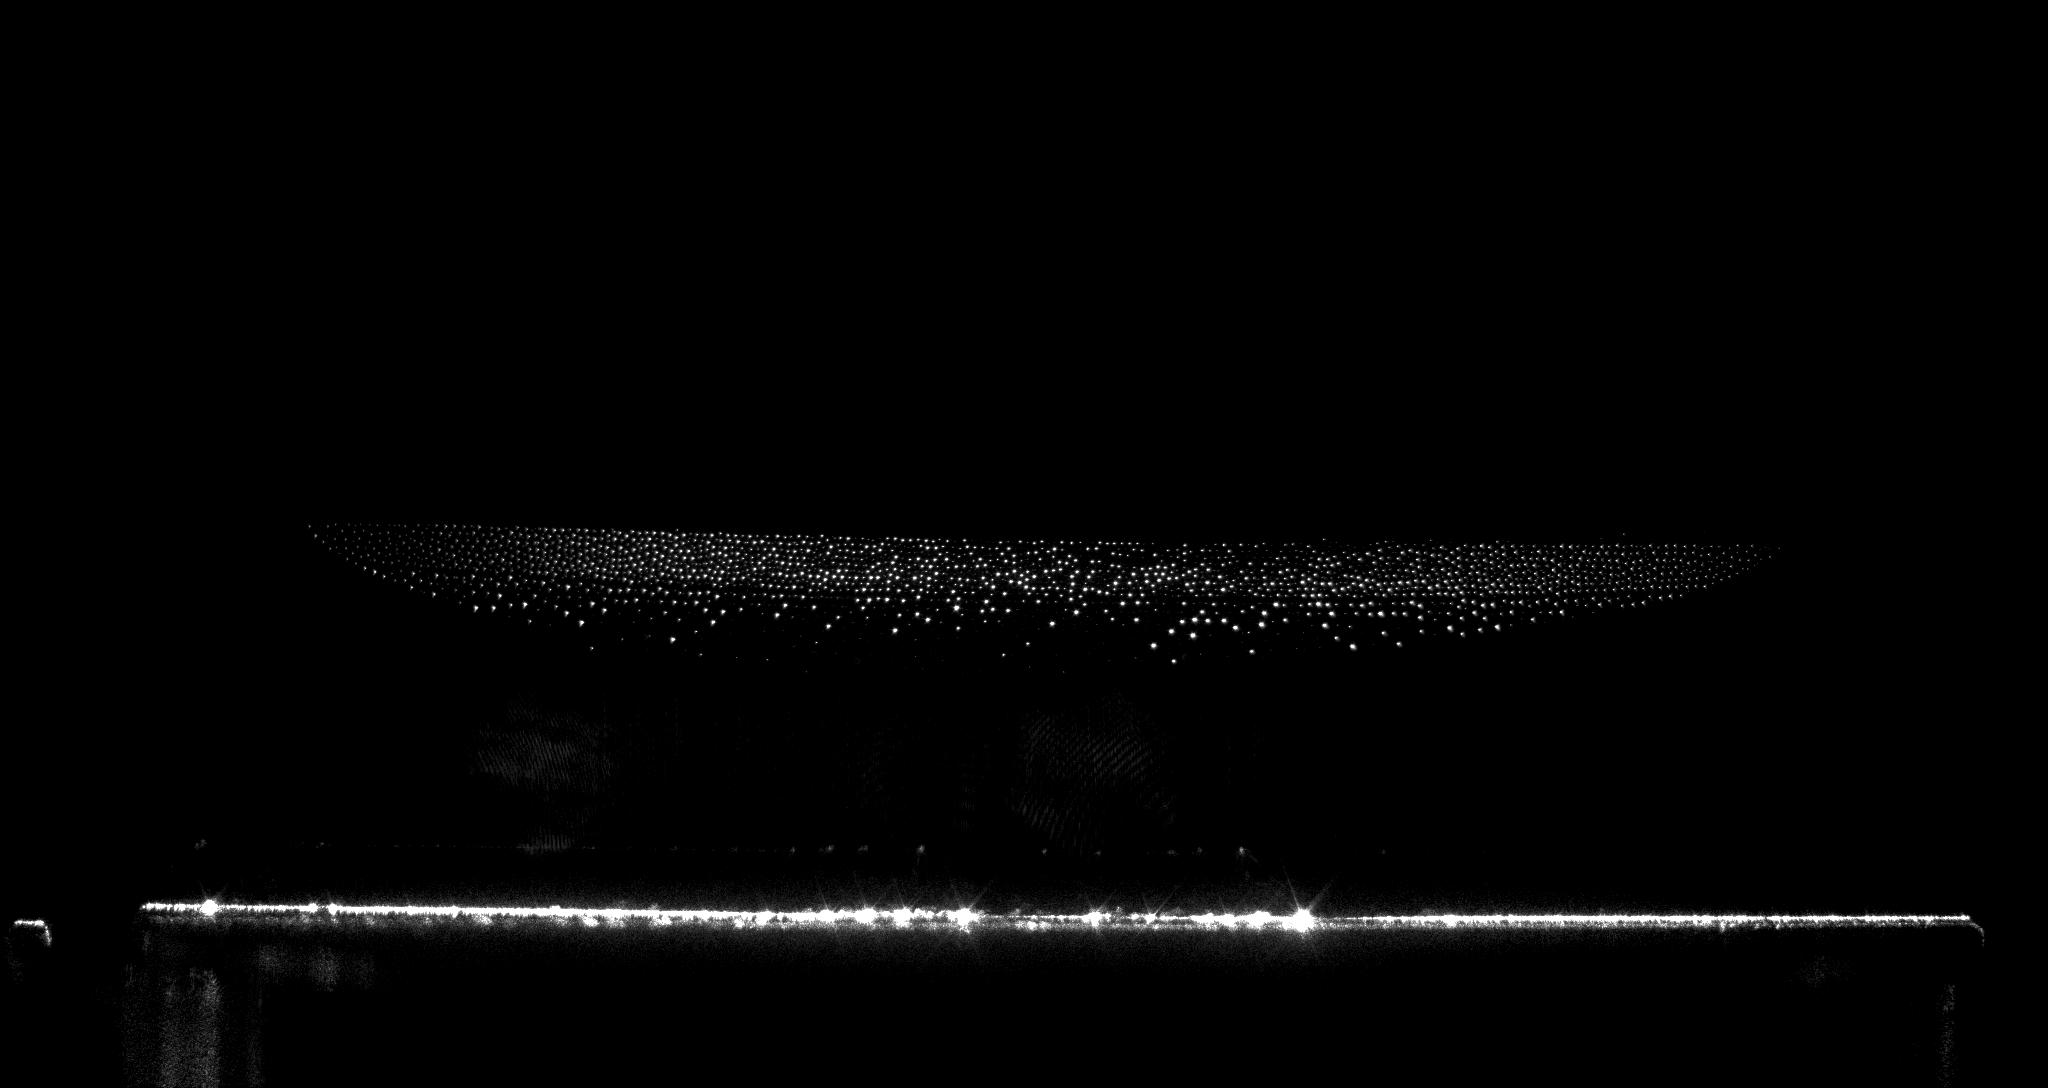
\includegraphics[width=\textwidth]{data/0,15V.jpg}
    \caption{Partikelwolke bei 0,15\,V}
    \label{fig:015v}
\end{figure}

\begin{figure}[ht]
    \centering
    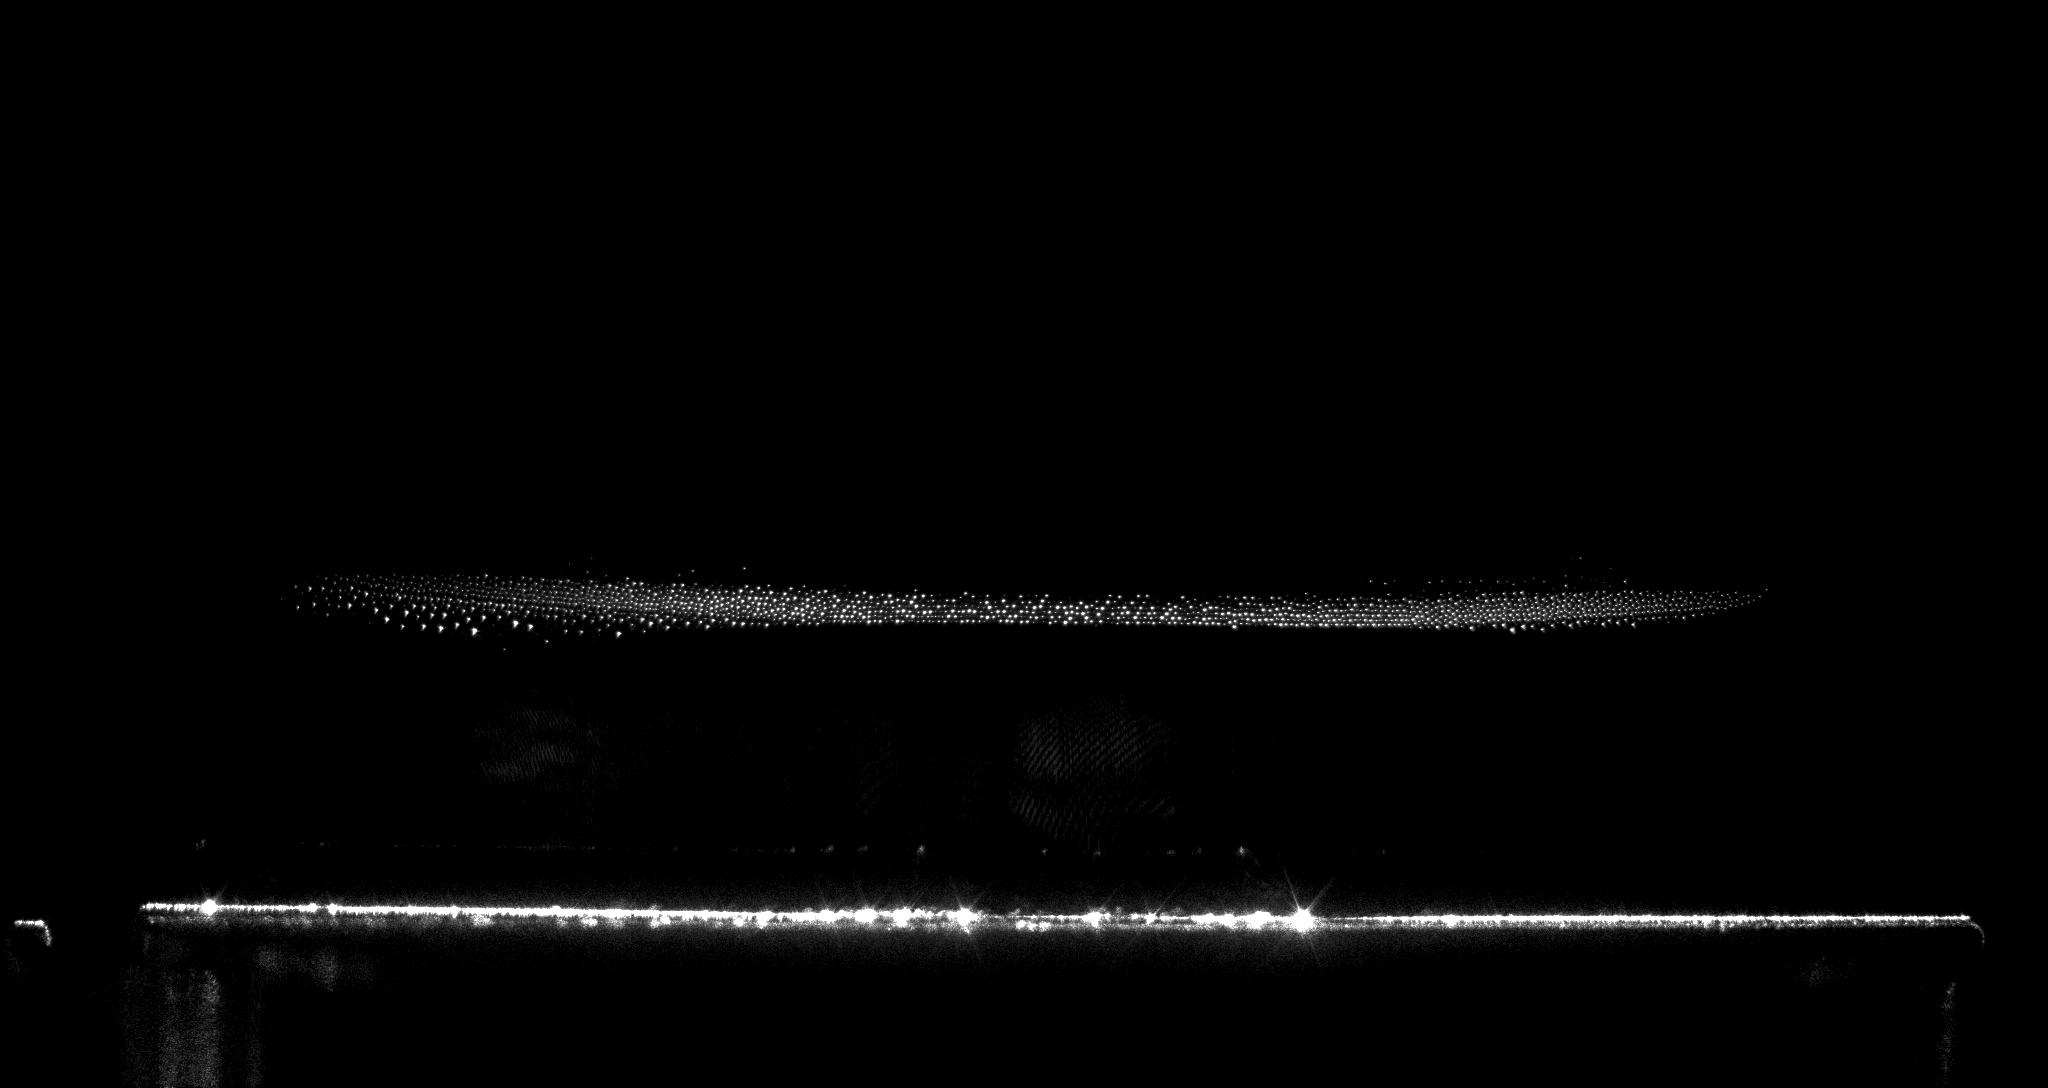
\includegraphics[width=\textwidth]{data/1,5V.jpg}
    \caption{Partikelwolke bei 1,5\,V}
    \label{fig:15v}
\end{figure}

Schlußendlich wird die Spannung in 0,01\,V Schritten heruntergefahren: Der Kristall erlangt zunächst wieder seine ursprünglichen Ausdehnungen. Bei einer Spannung von 0,11\,V ist das elektrische Feld nicht mehr stark genug um das Plasma zu erhalten und die Partikel stürzen aufgrund der Erdbeschleunigung abrupt herab.

\chapter{Fazit}
Alle theoretischen Überlegungen in der Vorbereitung sind mit unseren Messungen bestätigt. Der Versuch ist ein interessante Möglichkeit ein aktuelles Forschungsthema kennenzulernen und wurde erfolgreich durchgeführt. %\cleardoublepage

    % appendix for more or less interesting calculations
    \Appendix
    \chapter*{\appendixname} \addcontentsline{toc}{chapter}{\appendixname}
    % to make the appendix appear in ToC without number. \appendixname = 
    % Appendix or Anhang (depending on chosen language)
    
\section{Graphen}

\subsection{BCC-Gitter}

\begin{figure}[H]
\begin{minipage}[b]{0.3\textwidth}
    \centering
    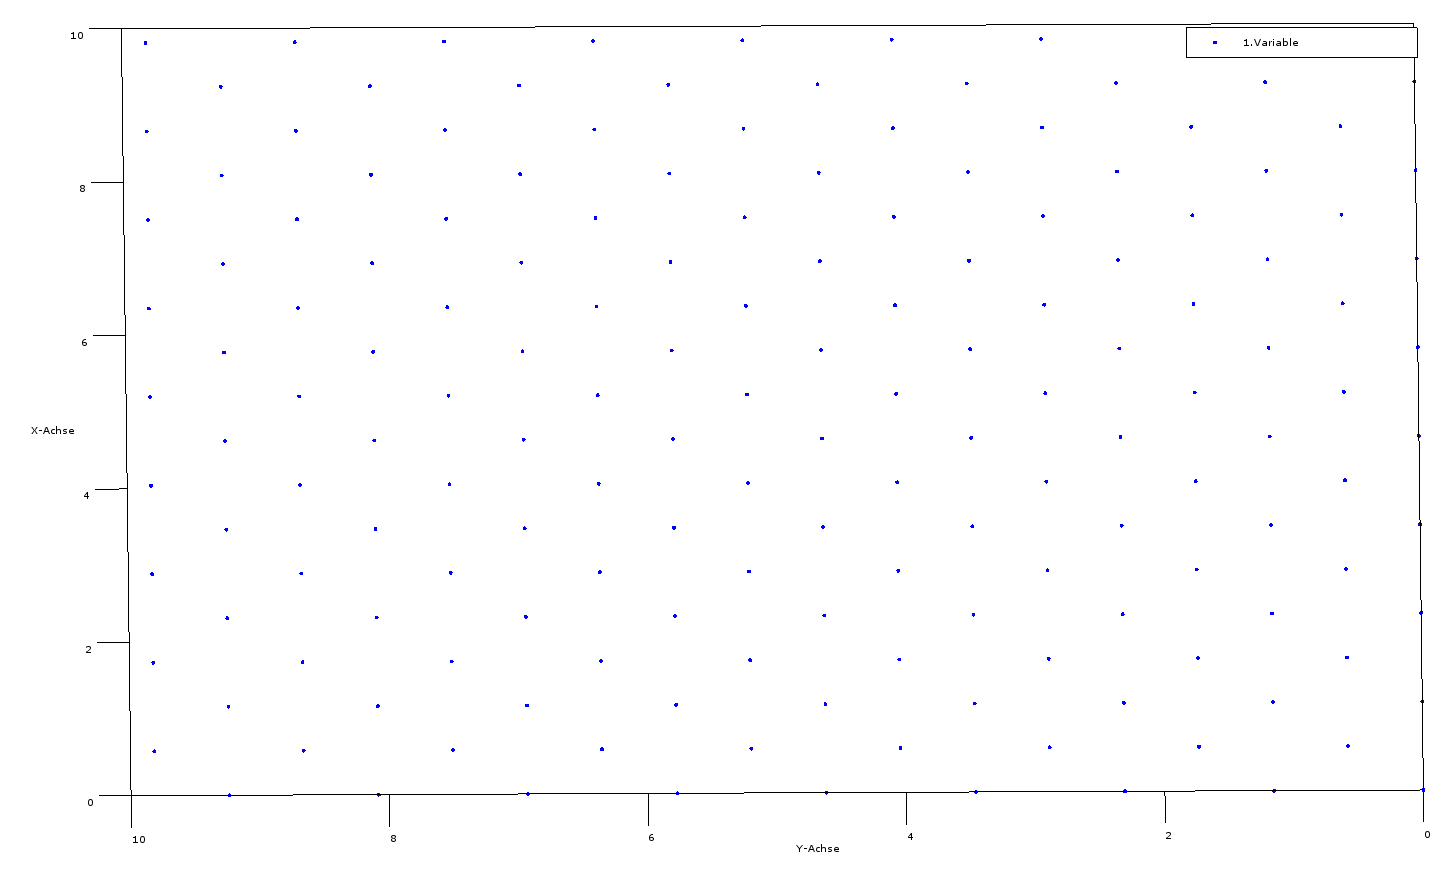
\includegraphics[scale=0.12]{data/bcc_x-y.PNG}
    \caption{BCC: xy-Ebene}
    \label{fig:bccxy}
\end{minipage}    
\begin{minipage}[b]{0.3\textwidth}
    \centering
    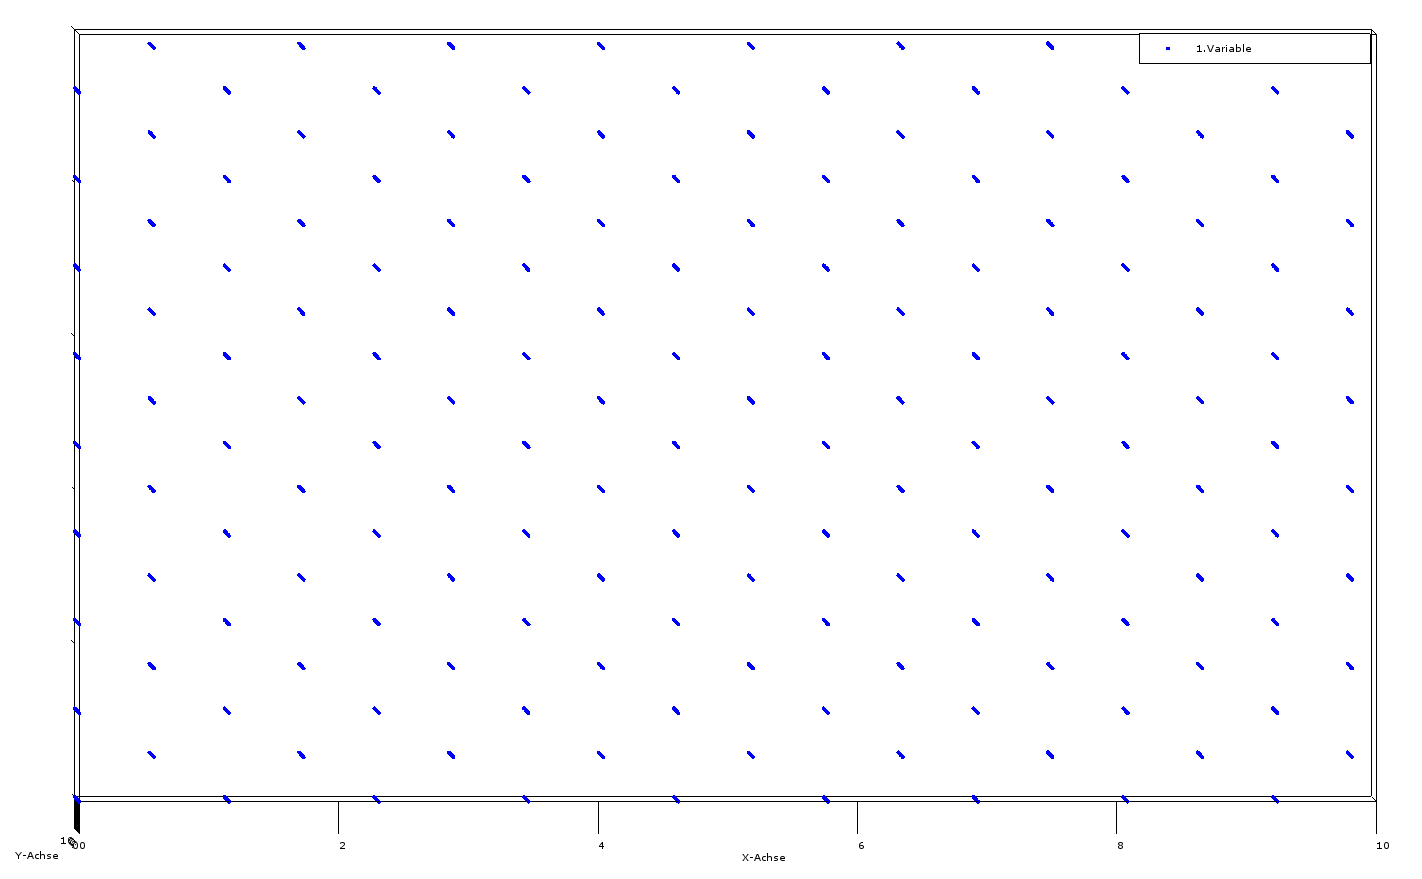
\includegraphics[scale=0.12]{data/bcc_x-z.PNG}
    \caption{BCC: xz-Ebene}
    \label{fig:bccxz}
\end{minipage} 
\begin{minipage}[b]{0.3\textwidth}
    \centering
    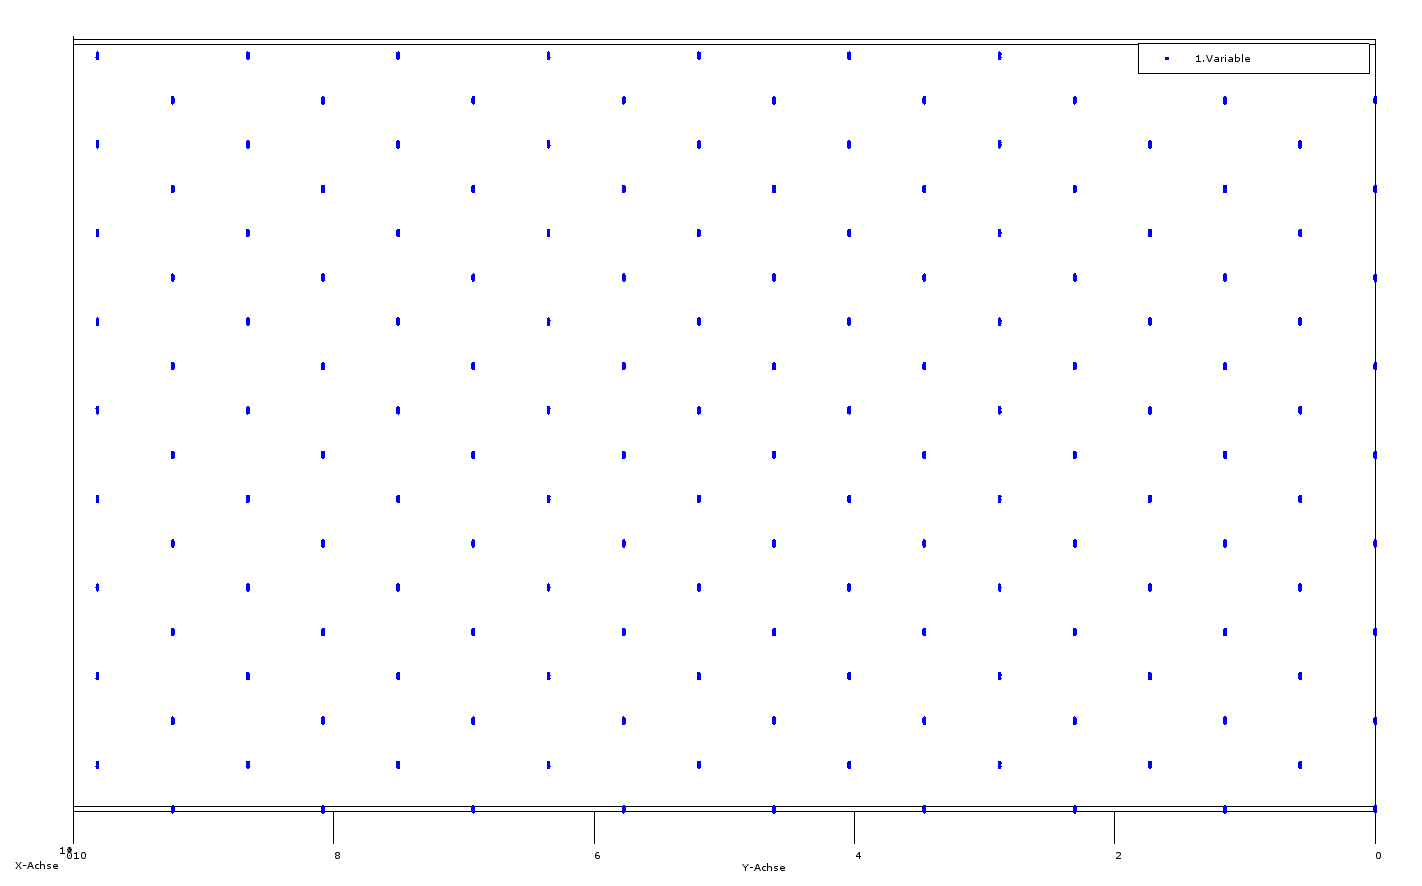
\includegraphics[scale=0.12]{data/bcc_y-z.PNG}
    \caption{BCC: yz-Ebene}
    \label{fig:bccyz}
\end{minipage} 
\end{figure}

\begin{figure}[H]
\begin{minipage}[b]{0.5\textwidth}
    \centering
    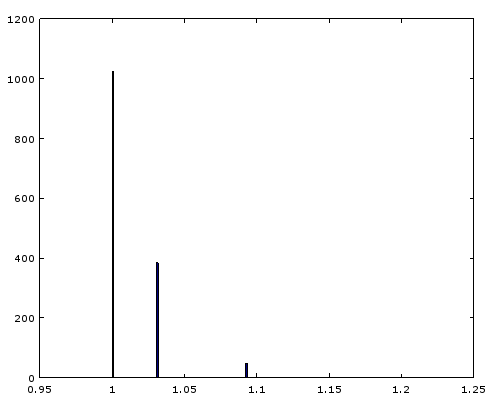
\includegraphics[scale=0.5]{data/bcc-hist.PNG}
    \caption{BCC: Teilchenabstände}
    \label{fig:bccabstand}
\end{minipage}    
\begin{minipage}[b]{0.5\textwidth}
    \centering
    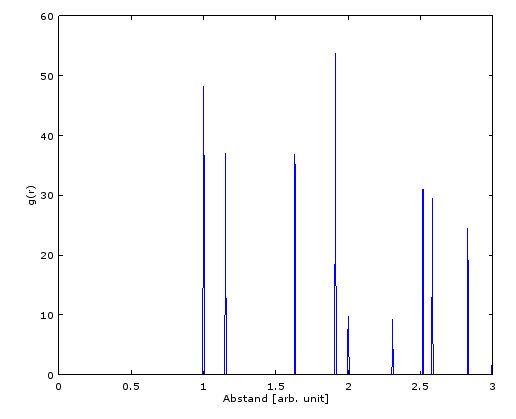
\includegraphics[scale=0.5]{data/bcc-paircorrelation.PNG}
    \caption{BCC: Paarkorrelationsfunktion}
    \label{fig:bccg}
\end{minipage} 
\end{figure}

\subsection{FCC-Gitter}

\begin{figure}[H]
\begin{minipage}[b]{0.3\textwidth}
    \centering
    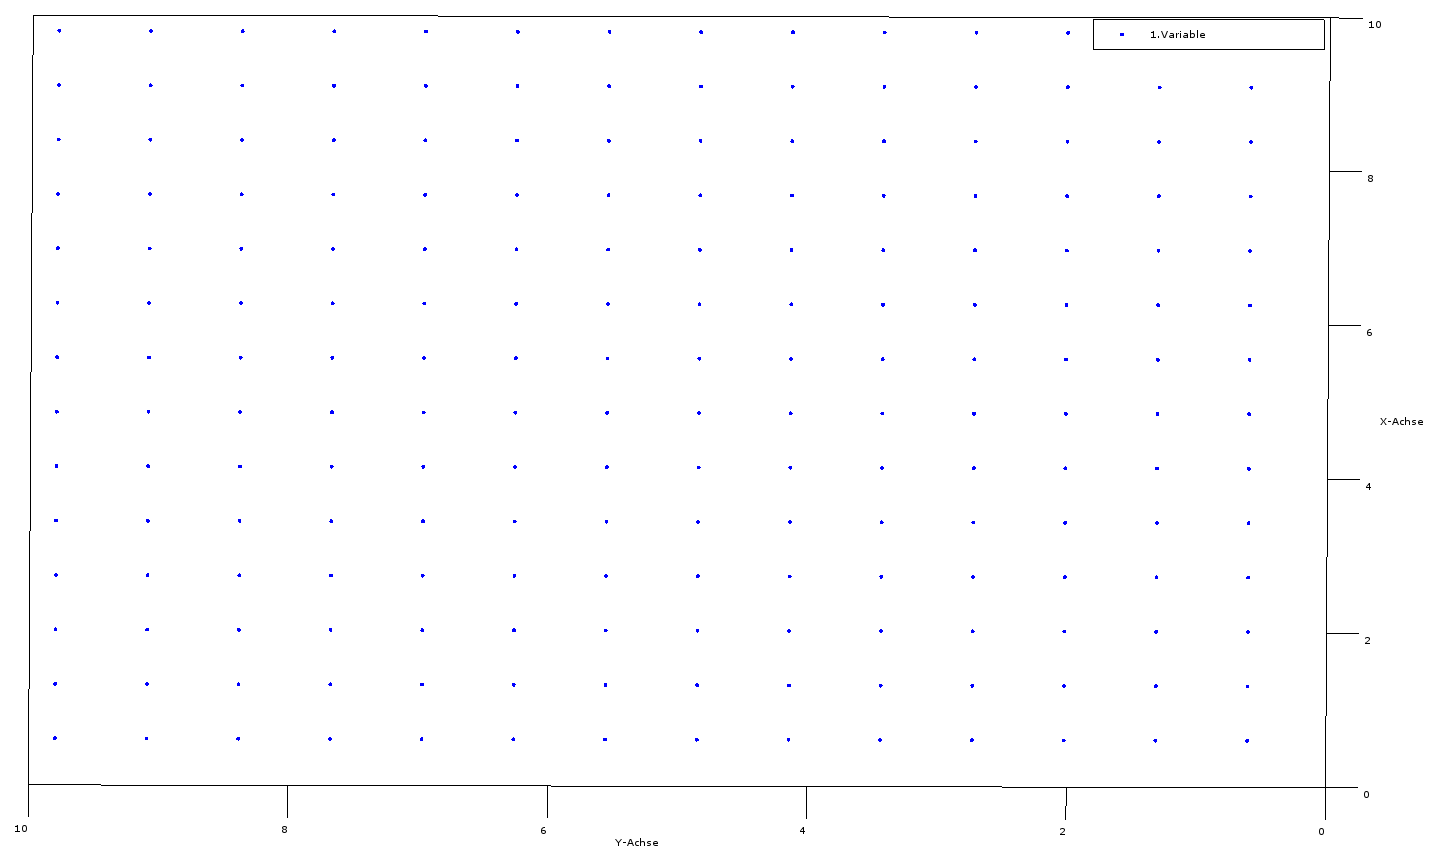
\includegraphics[scale=0.12]{data/fcc_x-y.PNG}
    \caption{FCC: xy-Ebene}
    \label{fig:fccxy}
\end{minipage}    
\begin{minipage}[b]{0.3\textwidth}
    \centering
    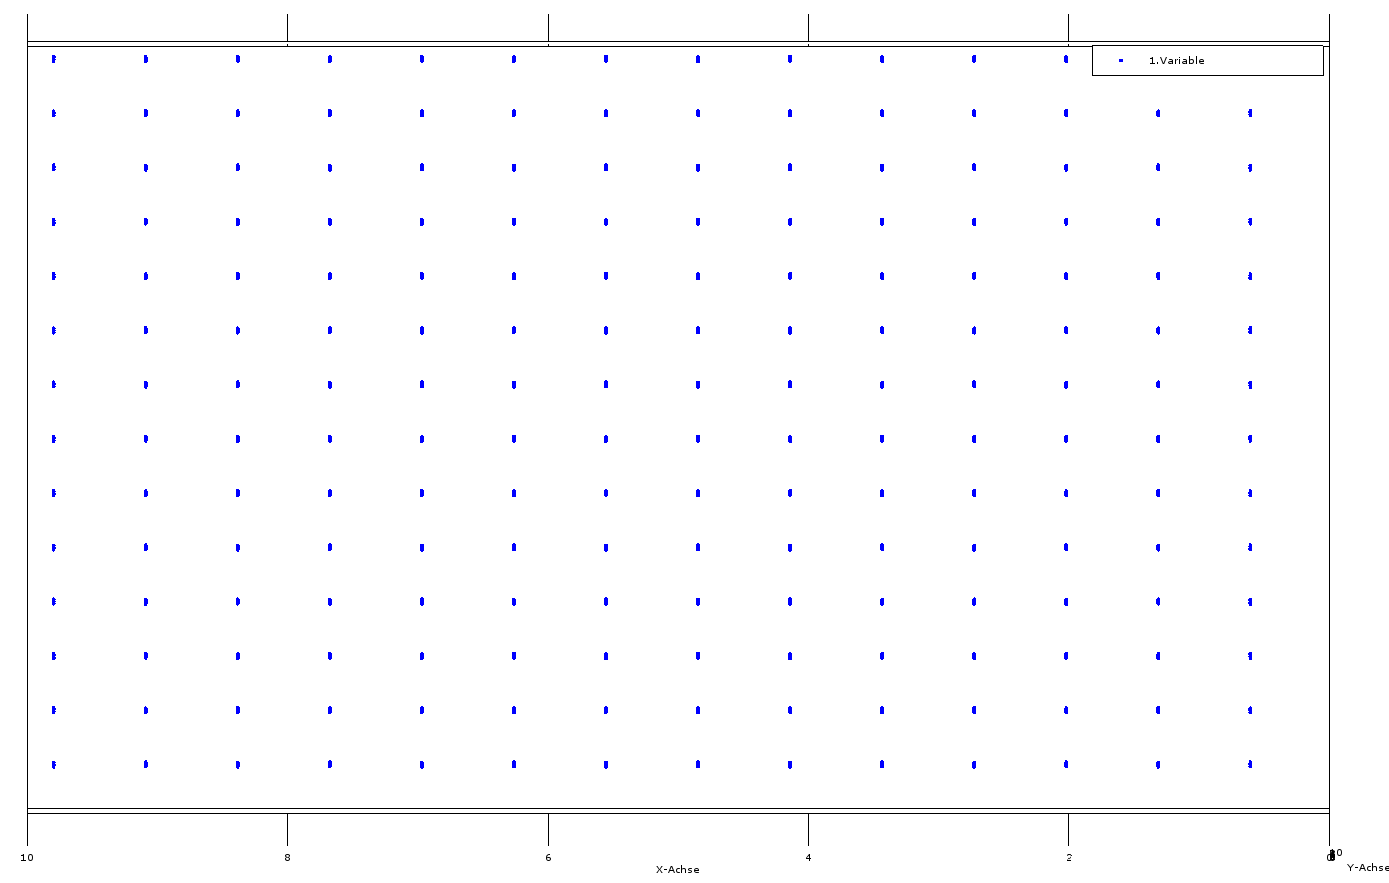
\includegraphics[scale=0.12]{data/fcc_x-z.PNG}
    \caption{FCC: xz-Ebene}
    \label{fig:fccxz}
\end{minipage} 
\begin{minipage}[b]{0.3\textwidth}
    \centering
    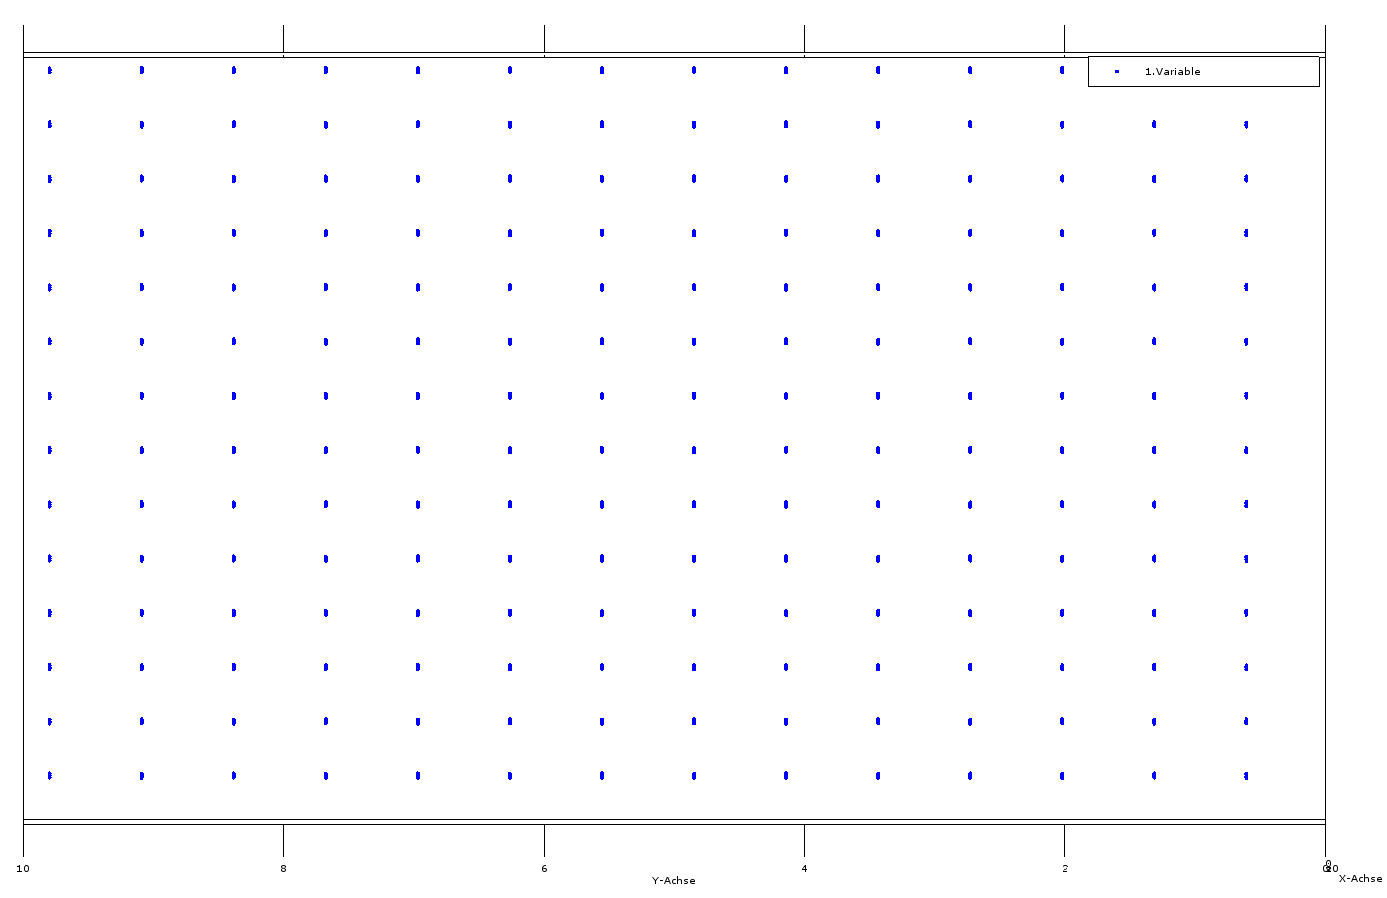
\includegraphics[scale=0.12]{data/fcc_y-z.PNG}
    \caption{FCC: yz-Ebene}
    \label{fig:fccyz}
\end{minipage} 
\end{figure}

\begin{figure}[H]
\begin{minipage}[b]{0.5\textwidth}
    \centering
    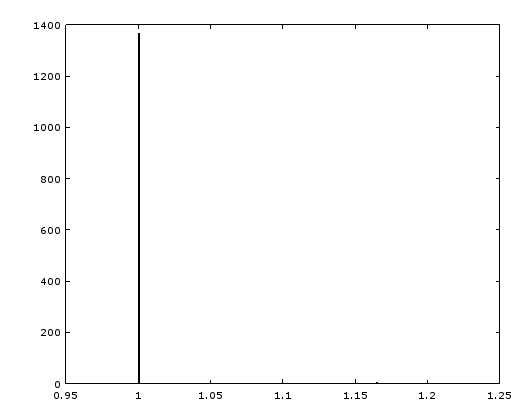
\includegraphics[scale=0.5]{data/fcc-hist.PNG}
    \caption{FCC: Teilchenabstände}
    \label{fig:fccabstand}
\end{minipage}    
\begin{minipage}[b]{0.5\textwidth}
    \centering
    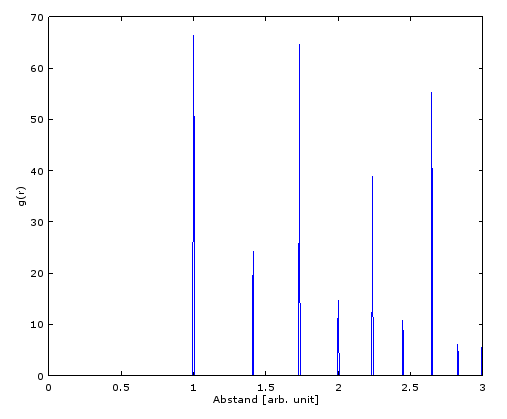
\includegraphics[scale=0.5]{data/fcc-paircorrelation.PNG}
    \caption{FCC: Paarkorrelationsfunktion}
    \label{fig:fccg}
\end{minipage} 
\end{figure}

\subsection{HCP-Gitter}

\begin{figure}[H]
\begin{minipage}[b]{0.3\textwidth}
    \centering
    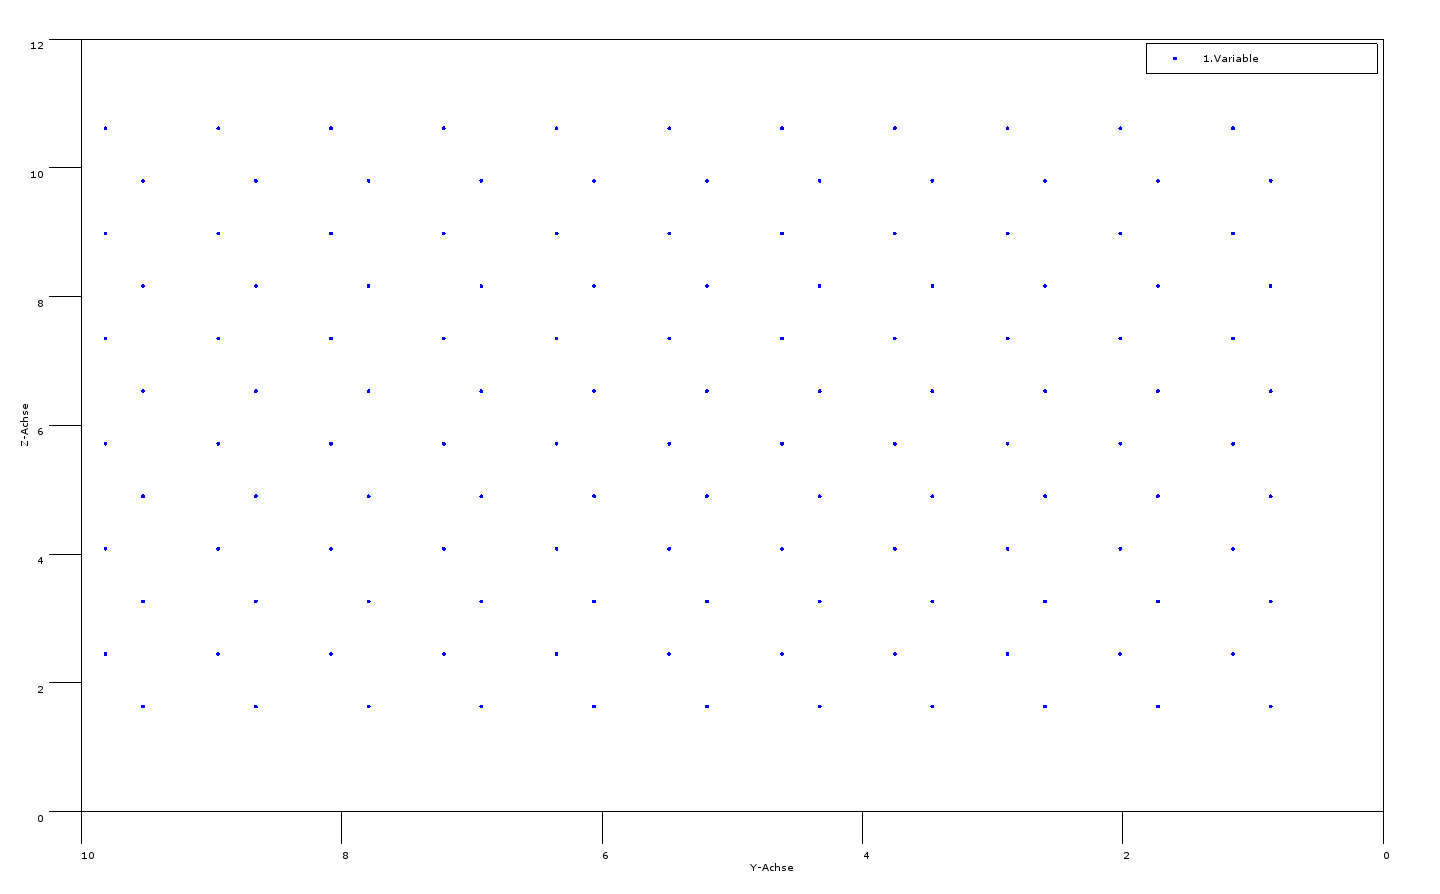
\includegraphics[scale=0.12]{data/hcp_x-y.PNG}
    \caption{HCP: xy-Ebene}
    \label{fig:hcpxy}
\end{minipage}    
\begin{minipage}[b]{0.3\textwidth}
    \centering
    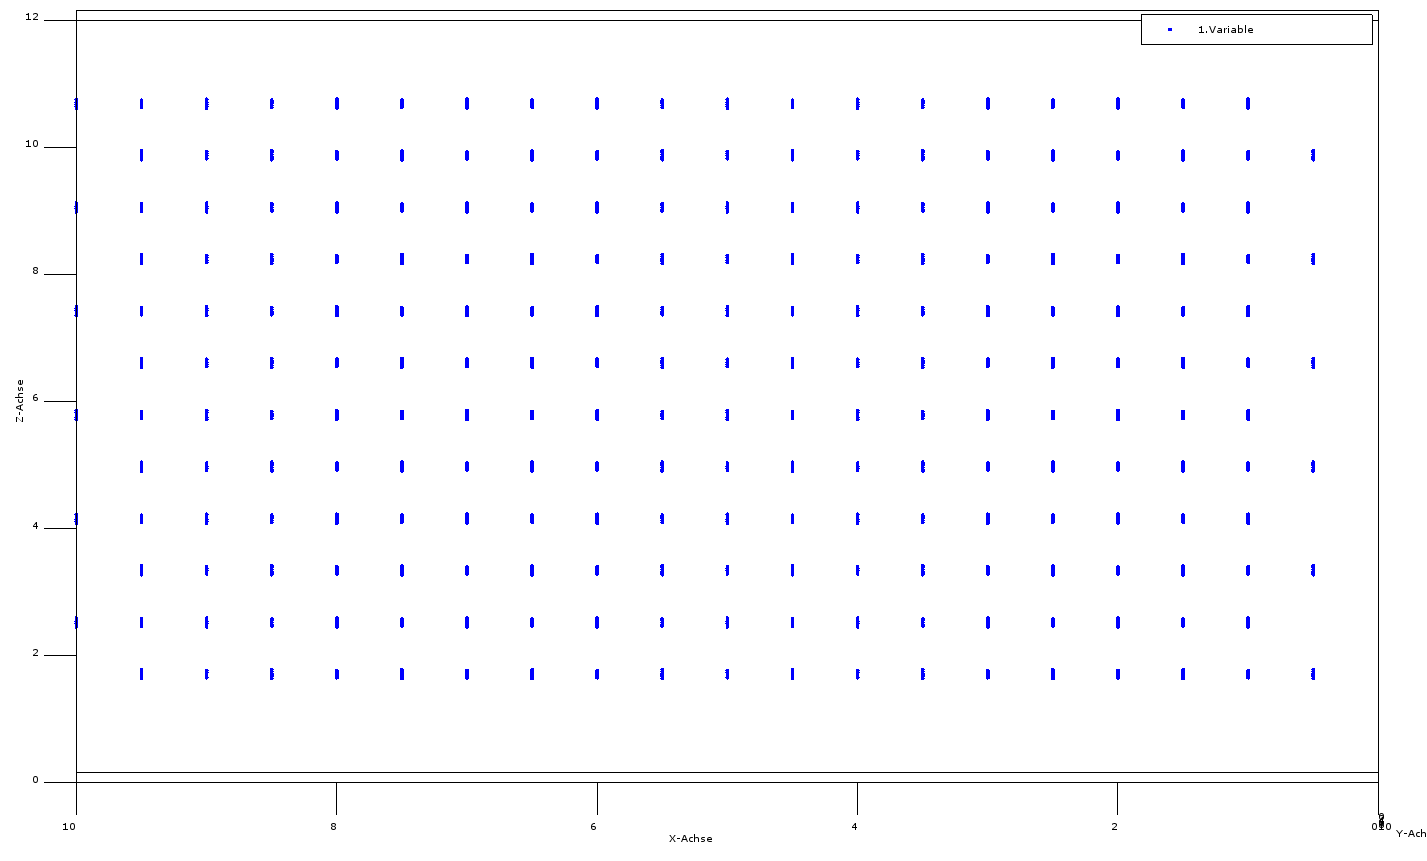
\includegraphics[scale=0.12]{data/hcp_z-x.PNG}
    \caption{HCP: xz-Ebene}
    \label{fig:hcpxz}
\end{minipage} 
\begin{minipage}[b]{0.3\textwidth}
    \centering
    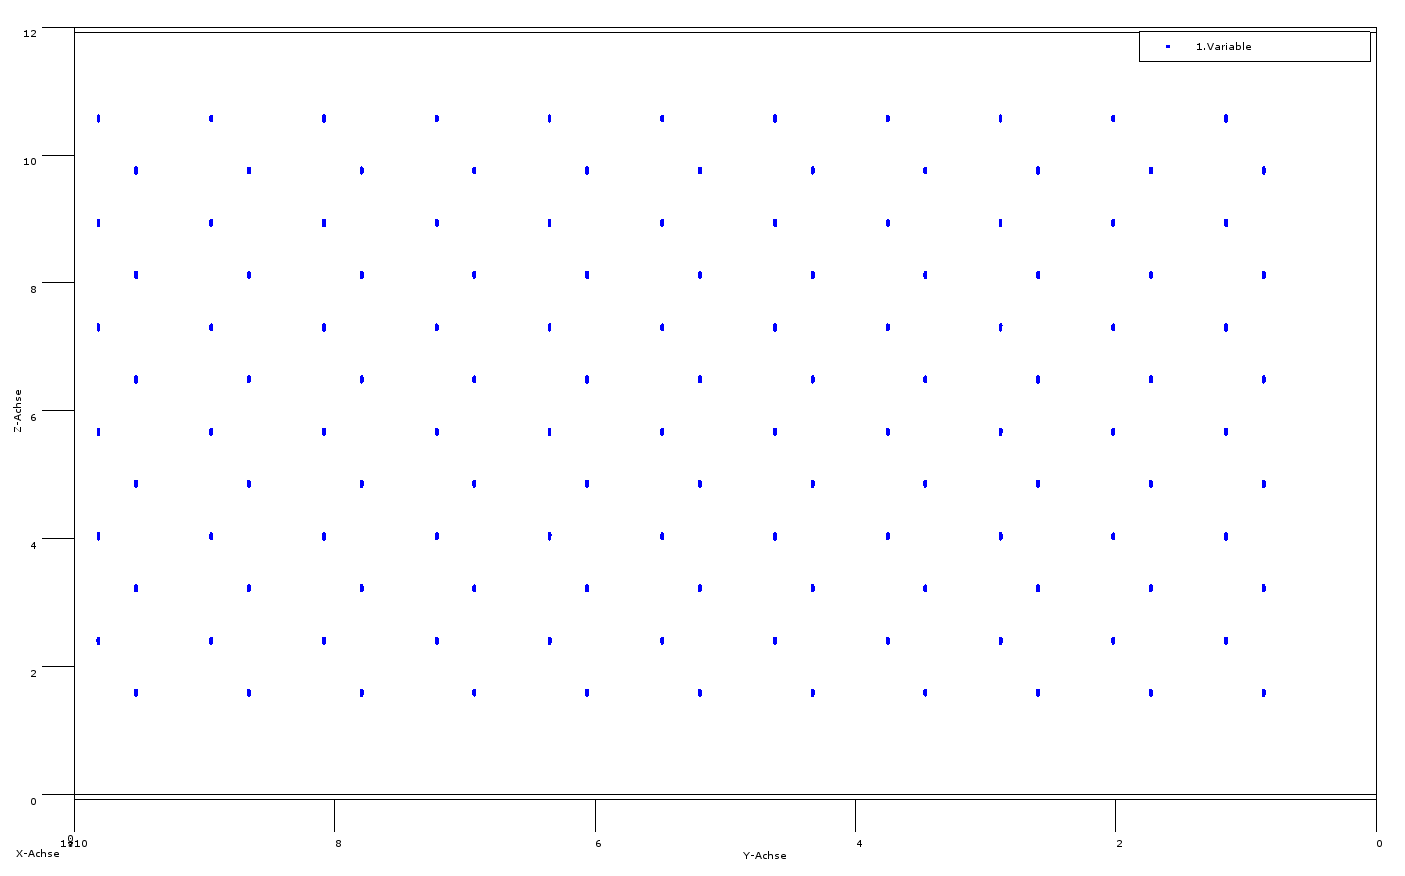
\includegraphics[scale=0.12]{data/hcp_z-y.PNG}
    \caption{HCP: yz-Ebene}
    \label{fig:hcpyz}
\end{minipage} 
\end{figure}

\begin{figure}[H]
\begin{minipage}[b]{0.5\textwidth}
    \centering
    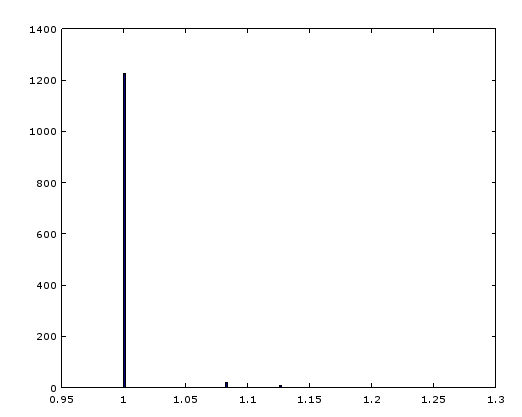
\includegraphics[scale=0.5]{data/hcp-hist.PNG}
    \caption{HCP: Teilchenabstände}
    \label{fig:hcpabstand}
\end{minipage}    
\begin{minipage}[b]{0.5\textwidth}
    \centering
    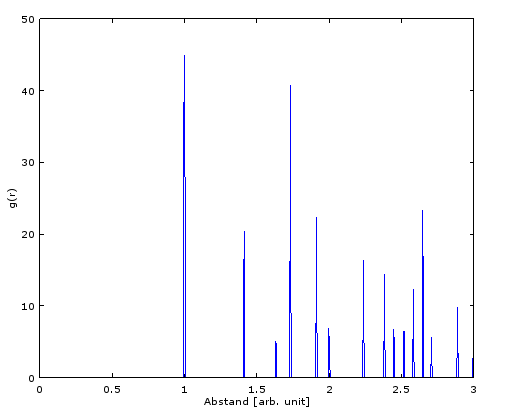
\includegraphics[scale=0.5]{data/hcp-paircorrelation.PNG}
    \caption{HCP: Paarkorrelationsfunktion}
    \label{fig:hcpg}
\end{minipage} 
\end{figure}










\FloatBarrier
\pagebreak
\newpage
\begin{landscape}
\section{Messwerte}

\begin{table}[H]
\begin{tabular}{|l|llll|l|l|}
    \multicolumn{7}{l}{Horizontale Abstände}\\ \hline
     &Mitte – unten &Mitte - halbe Höhe &Halber Radius – unten &halber Radius - halbe Höhe & &\\ \hline
     &6.75 &8 &8.36 &8.5016 & &\\
     &7.125 &8.75 &8.2971 &9.2525 & &\\
     &7.6833 &9.75 &8.4 &9.208 &Mittelwert: &Anzahl:\\\hline
    Mittelwerte: &7.19 &8.83 &8.35 &8.99 &8.34 &192.57894\\\hline
    \multicolumn{7}{l}{}\\
    \multicolumn{7}{l}{Vertikale Abstände}\\ \hline
     &6.3433 &6.8333 &6.4 &6.604 & &\\
     &6.6 &6.2 &5.2 &7.2 & &\\
     &5.25 &5.8333 &5.75 &7.755 &Mittelwert: &Anzahl:\\\hline
    Mittelwerte: &6.06 &6.29 &5.78 &7.19 &6.33 &146.16603\\\hline
\end{tabular}
\caption{Messwerte zur Anzahlbestimmung}
\label{tab:mess-anz}
\end{table}

\begin{table}[H]
\begin{tabular}{|l|l|l|} \hline
Horizontale Weite in mm ???& Horizontale Anzahl & Anzahl Grundfläche \\
1409 & 168.94 & 22415.83 \\ \hline
vertikale Weite in mm ???& vertikale Anzahl & Anzahl Volumen \\ 
120 & 18.96 & \cellcolor[HTML]{C0C0C0}{\color[HTML]{FD6864} 425004} \\ \hline
\end{tabular}
\caption{Anzahlbestimmung}
\label{tab:anz}
\end{table}
\end{landscape}

\pagebreak
 %\cleardoublepage



    % Bibliography
    \TheBibliography

    % BIBTEX
    % use if you want citations to appear even if they are not referenced to: 
    % \nocite{*} or maybe \nocite{Kon64,And59} for specific entries
    %\nocite{*}
    \nocite{*}
    \bibliographystyle{unsrt}
    \bibliography{lit.bib}

    % THEBIBLIOGRAPHY
    %\begin{thebibliography}{000}
    %    \bibitem{ident}Entry into Bibliography.
    %\end{thebibliography}
\end{document}
